% !Mode:: "TeX:UTF-8"
% !TEX program  = xelatex
% !BIB program  = biber
\documentclass[AutoFakeBold,AutoFakeSlant,language=chinese,degree=bachelor,zihao=-4]{sustechthesis}
% 1. AutoFakeBold 与 AutoFakeSlant 为伪粗与伪斜,如果本机上有相应粗体与斜体字体,请使用 xeCJK 宏包进行设置,例如:
%   \setCJKmainfont[
%     UprightFont = * Light,
%     BoldFont = * Bold,
%     ItalicFont = Kaiti SC,
%     BoldItalicFont = Kaiti SC Bold,
%   ]{Songti SC}
%
% 2. language=chinese 基于为 ctexart 文类提供的中文排版方案修改,如果使用英文进行论文创作,请使用 language=english 选项。
%
% 3. degree=bachelor 为 sustechthesis 文类提供的本科生毕业论文模板,其他可选项为 master 与 doctor,但是均未实现,如果您对此有兴趣,欢迎 PR。
%
% 4. sustechthesis.cls 文类主要参考自去年完成使命的 sustechthesis.tex,在这一年的时间,作者的 TeX 风格与常用宏包发生许多变化,因为之前的思想为仅提供必要的格式修改相关代码,所以转换为文类形式所进行的修改较少,而近期的风格与常用宏包均体现在以下的例子文件中。
%
% 5. 示例文件均放置于相应Catalog的 examples 文件夹下,构建自己论文时可暂时保留,用以检索接口与使用方法。
%
% 6. 英文Catalog需要居中可以使用:\renewcommand{\contentsname}{\centerline{Content}}
%
% 7. LaTeX 中公式编号括号样式及章节关联的方法:https://liam.page/2013/08/23/LaTeX-Formula-Number/

% !Mode:: "TeX:UTF-8"
% !TEX program  = xelatex

% 数学符号与环境
\usepackage{amsmath,amssymb}
  \newcommand{\dd}{\mathrm{d}}
  \newcommand{\RR}{\mathbb{R}}
% Reference
\usepackage[style=gb7714-2015,gbpub=false]{biblatex}
  \addbibresource{ref.bib}
% 无意义文本
\usepackage{zhlipsum,lipsum}
% 列表环境设置
\usepackage{enumitem}
% 浮动题不越过 \section
\usepackage[section]{placeins}
% 超链接
\usepackage{hyperref}
% 图片,子图,浮动题设置
\usepackage{graphicx,subcaption,float}
% 抄录环境设置,更多有趣例子请命令行输入 `texdoc tcolorbox`
\usepackage{tcolorbox}
  \tcbuselibrary{xparse}
  \DeclareTotalTCBox{\verbbox}{ O{green} v !O{} }%
    {fontupper=\ttfamily,nobeforeafter,tcbox raise base,%
    arc=0pt,outer arc=0pt,top=0pt,bottom=0pt,left=0mm,%
    right=0mm,leftrule=0pt,rightrule=0pt,toprule=0.3mm,%
    bottomrule=0.3mm,boxsep=0.5mm,bottomrule=0.3mm,boxsep=0.5mm,%
    colback=#1!10!white,colframe=#1!50!black,#3}{#2}%
\tcbuselibrary{listings,breakable}
  \newtcbinputlisting{\Python}[2]{
    listing options={language=Python,numbers=left,numberstyle=\tiny,
      breaklines,commentstyle=\color{white!50!black}\textit},
    title=\texttt{#1},listing only,breakable,
    left=6mm,right=6mm,top=2mm,bottom=2mm,listing file={#2}}
% 三线表支持
\usepackage{booktabs}

% LaTeX logo
\usepackage{hologo}

% \usepackage{algorithm}
% \usepackage{algpseudocode}
% \usepackage{amsmath}
% \renewcommand{\algorithmicrequire}{\textbf{Input:}}
% \renewcommand{\algorithmicensure}{\textbf{Output:}}


% \State <text>
% \If{<condition>} <text> \EndIf
% \If{<condition>} <text> \Else <text> \EndIf
% \If{<condition>} <text> \ElsIf{<condition>}  <text> \Else <text> \EndIf
% \For{<condition>} <text> \EndFor
% \ForAll{<condition>} <text> \EndFor
% \While{<condition>} <text> \EndWhile
% \Repeat <text> \Until{<condition>}
% \Loop <text> \EndLoop
% \Require <text>
% \Ensure <text>
% \Function{<name>}{<params>} <body> \EndFunction
% \State \Return <text>
% \Comment{<text>}

% \usepackage{algorithm}  
% \usepackage{algorithmicx}  
% \usepackage{algpseudocode}
% \makeatletter
% \newenvironment{breakablealgorithm}
%   {% \begin{breakablealgorithm}
%    \begin{center}
%      \refstepcounter{algorithm}% New algorithm
%      \hrule height.8pt depth0pt \kern2pt% \@fs@pre for \@fs@ruled
%      \renewcommand{\caption}[2][\relax]{% Make a new \caption
%        {\raggedright\textbf{\ALG@name~\thealgorithm} ##2\par}%
%        \ifx\relax##1\relax % #1 is \relax
%          \addcontentsline{loa}{algorithm}{\protect\numberline{\thealgorithm}##2}%
%        \else % #1 is not \relax
%          \addcontentsline{loa}{algorithm}{\protect\numberline{\thealgorithm}##1}%
%        \fi
%        \kern2pt\hrule\kern2pt
%      }
%   }{% \end{breakablealgorithm}
%      \kern2pt\hrule\relax% \@fs@post for \@fs@ruled
%    \end{center}
%   }
% \makeatother

\usepackage{algorithm}
\usepackage{algorithmic}

\renewcommand{\algorithmicrequire}{\textbf{Input:}}
\renewcommand{\algorithmicensure}{\textbf{Output:}}
\renewcommand\tablename{Table}

\captionsetup[figure]{labelfont={bf},labelformat={default},labelsep=period,name={Figure}}

% \addbibresource{ref.bib}

\usepackage{url}

\usepackage{multirow}
\usepackage{bm} % 导言区
% !Mode:: "TeX:UTF-8"
% !TEX program  = xelatex
\设置信息{
    % 键 = {{中文值}, {英文值}},
    分类号 = {{}, {}},
    编号 = {{}, {}},
    UDC = {{}, {}},
    密级 = {{}, {}},
    % 仅题目(不含副标题)、系别、专业,支持手动 \\ 换行,不支持自动换行。 Dense Prediction APP Based on Feature\mbox{-}aligned Pyramid Network
    题目 = {{基于Feature\mbox{-}aligned Pyramid }, {Dense Prediction APP Based on }},
    % 如无需副标题,删除值内容即可,不可删除键定义。
    副标题 = {{Network的密集预测APP设计}, {Feature\mbox{-}aligned Pyramid Network}},
    姓名 = {{赵奕帆}, {Yifan Zhao}},
    学号 = {{11812020}, {11812020}},
    系别 = {{计算机科学与工程系}, {Computer Science and Engineering}},
    专业 = {{计算机科学与技术}, {Computer Science and Technology}},
    指导老师 = {{程然}, {Ran Cheng}},
    时间 = {{2022年6月2日}, {June 2, 2022}},
    职称 = {{副教授}, {Associate Professor}},
    % 职称 = {{}, {}},
}
 % 论文信息
\begin{document}

% \中文标题页
\英文标题页

% \中文诚信承诺书
% \英文诚信承诺书

\前序格式化
\摘要标题
% !Mode:: "TeX:UTF-8"
% !TEX program  = xelatex
\begin{英文摘要}{Dense Prediction, Neural Networks, Feature Aligned, Android}
  Dense prediction is an important problem in the field of computer vision, which has important value for the segmentation and understanding of images in the fields of automatic driving, medical image recognition, etc.; it includes semantic segmentation, instance segmentation, panoptic segmentation, and other sub-tasks. In recent years, breakthroughs have been made in this problem by using neural networks. However, in the process of upsampling the upper convolutional layer using interpolation, there is a problem that the features obtained by the upsampling are not aligned with the features of the bottom-up convolutional layer. For this problem, this paper reproduces the feature alignment module and feature selection module in the FaPN(Feature-aligned Pyramid Network) to selects and aligns the key features of the upper convolutional layer through the contextual information before and after upsampling. Validation of the COCO2017 dataset confirms the module's performance for small objects and object boundary prediction. Modularized it to develop a simple Android app. The server side provides services by loading pre-trained models, and the client provides an easy-to-use UI interface and related functions required by various types of users. App has the function of quickly segmenting images and the characteristics of simple operation and flexible operation, which has certain practical value.
\end{英文摘要}

\begin{中文摘要}{密集预测;神经网络 ;特征对齐 ;安卓}
  密集预测是计算机视觉领域下的一类重要问题,这个问题对于自动驾驶,医学图像识别等领域的图像进行分割和理解具有重要价值;其包含了语义分割、实例分割、全景分割等多个子任务,近年来人们利用神经网络在这一问题上取得了突破。但在对于上卷积层利用插值法进行上采样的过程中,存在上采样得到的特征未与自下而上的卷积层的特征对齐的问题。对于这个问题,本文复现了FaPN(Feature-aligned Pyramid Network)中的特征对齐模块和特征选择模块,通过上采样前后的上下文信息对于上卷积层的关键特征进行选择和对齐。通过在COCO2017数据集上进行验证证实了模块对于小物体和物体边界预测的性能。并将其模块化,开发了一款简单的安卓APP。服务器端通过载入预训练模型提供服务,客户端提供了简单易用的UI界面和各类用户所需的相关功能。APP具有快速分割图像的功能和使用简单操作灵活的特点,具有一定的实用价值。
\end{中文摘要}


 % 论文摘要

\Catalog\clearpage % Catalog及换页

\正文格式化
% !Mode:: "TeX:UTF-8"
% !TEX program  = xelatex
\section{Introduction}
% 研究的目的、背景;理论依据、实验基础和研究方法或实验设计;预期结果和意义等
\subsection{Dense Prediction Tasks} 
With the rapid development of computer science research and related industries in recent years, people's production and lifestyle have undergone tremendous changes. Breakthroughs have been made in artificial intelligence, especially in the field of machine learning, and it has also been applied in more and more fields.

Neural networks have made impressive results in a variance of tasks \cite{multivandenhende2021}, such as semantic segmentation \cite{long2015fully}, instance segmentation \cite{he2017mask}, augmented reality \cite{abu2018augmented} and panoptic segmentation \cite{kirillov2019panoptic}. All of them are part of a dense prediction task, a collection of computer vision tasks aiming at labeling every pixel in the given image into a predefined class \cite{huang2021fapn}.


\begin{figure}[htb]
    \centering
    \begin{subfigure}[t]{.45\linewidth}
        \centering
        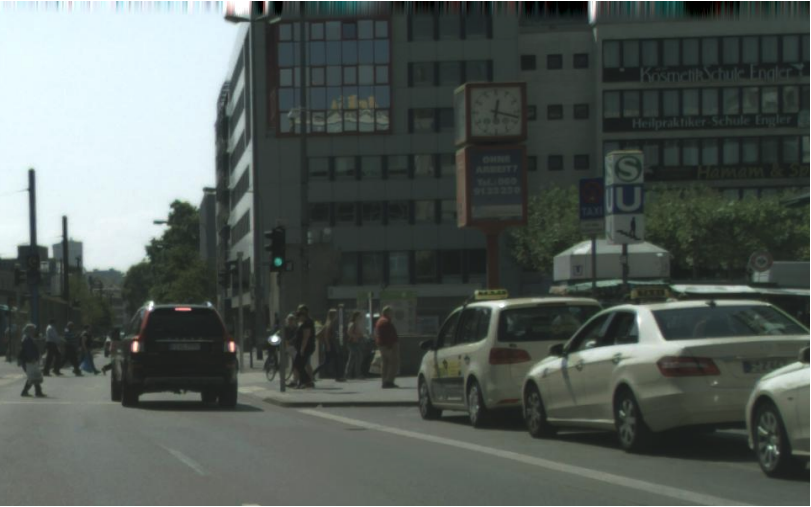
\includegraphics[width=1\textwidth]{figures/RawImage.png}
        \caption{Raw Image}\label{Raw Image}
    \end{subfigure}
    \begin{subfigure}[t]{.45\linewidth}
        \centering
        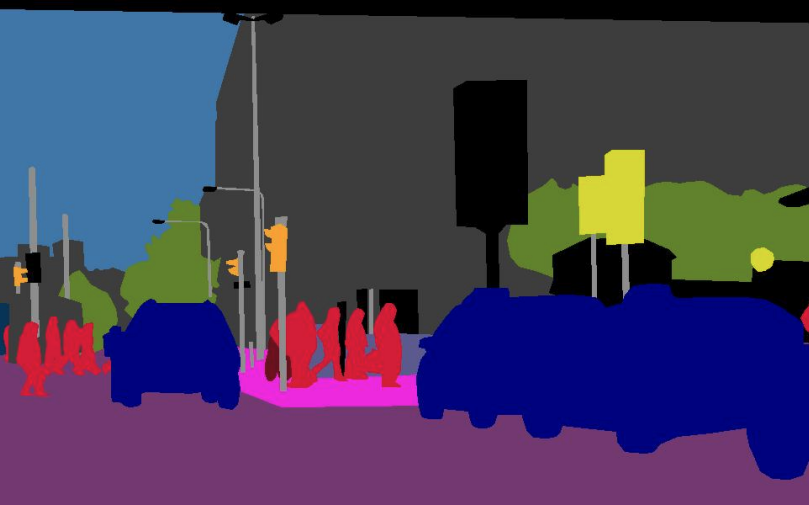
\includegraphics[width=1\textwidth]{figures/Semantic Segmentation2.png}
        \caption{Semantic Segmentation}\label{Semantic Segmentation}
    \end{subfigure}
    \begin{subfigure}[t]{.45\linewidth}
        \centering
        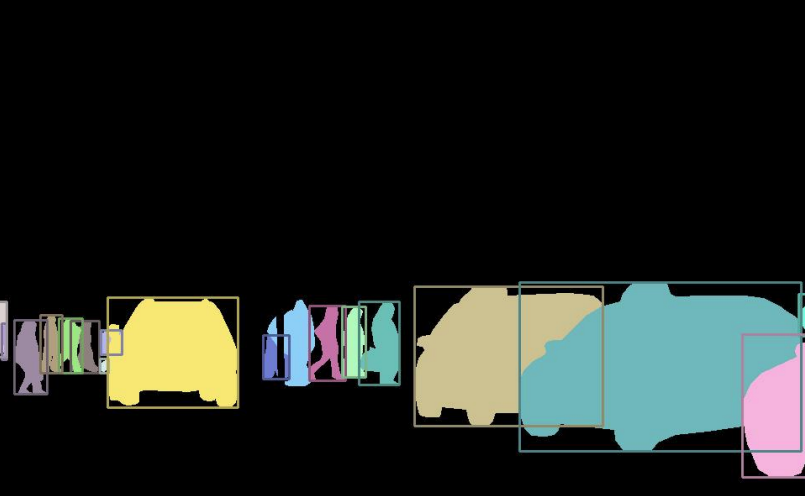
\includegraphics[width=1\textwidth]{figures/Instance Segmentation2.png}
        \caption{Instance Segmentation}\label{Instance Segmentation}
    \end{subfigure}
    \begin{subfigure}[t]{.45\linewidth}
        \centering
        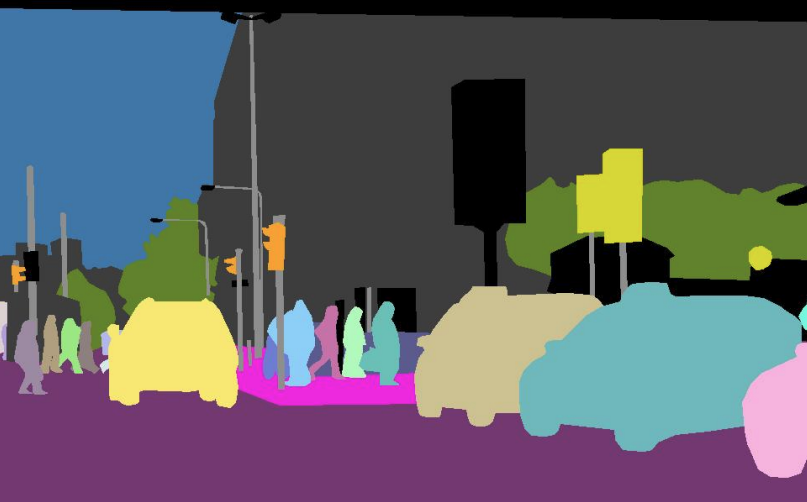
\includegraphics[width=1\textwidth]{figures/PanopticSegmentation.png}
        \caption{Panoptic Segmentation}\label{Panoptic Segmentation}
    \end{subfigure}
    \caption{Computer vision tasks \cite{kirillov2019panoptic}: For a given a) raw image, b) Semantic Segmentation, c) Instance Segmentation, d) Panoptic Segmentation are a part of a dense prediction task, aiming at labeling every pixel in the given image into a predefined class. Panoptic segmentation was proposed by Alexander Kirillov et al. in 2018.}\label{Dense Prediction Tasks}
\end{figure}


Any of these tasks is one of the basic problems of computer vision and has a very high value of use, so it has high importance in various applications, such as autonomous driving \cite{de2017semantic}, medical image segmentation \cite{lei2020medical}, and geospatial object segmentation \cite{zheng2020foreground}.

% Dense prediction可以被视作图像分类任务和目标检测任务的综合任务,其同时需要图像中物体的语义信息和位置信息。为了同时获取两类信息并进行对齐,大多数网络采取了top-down feature pyramid的网络架构。这类网络架构可以获取给定图像不同层级的语义信息;底层网络得到的图像分辨率较高,主要用来获取instance的位置信息;高层图像得到的图像分辨率较低,包含更多抽象的语义信息,用以预测小物体和判断物体边缘的位置。
Dense prediction can be regarded as a comprehensive task of image classification task and object detection task, it needs both semantic information and position information of instances in the given images. To obtain two kinds of information and align them at the same time, most networks adopt the network architecture of the top-down feature pyramid. This type of network architecture can obtain semantic information at different levels of a given image; the image obtained by the lower-level convolution layers has a higher resolution and is mainly used to obtain the location information of the instance; the image obtained by the high-level image has a lower resolution and contains more abstract semantics information for predicting small objects and judging the location of object edges.


\subsection{Apply Dense Prediction on Mobile Terminal} 

Despite all the success mentioned above, most works mainly focuses on applications on server clusters that need powerful computational resources, beyond the capabilities of the mobile terminal, such as mobile phones and embedded devices \cite{zhang2022topformer}. However, in the past few years, the resolution and imaging capabilities of mobile terminal cameras have been significantly improved, meanwhile, mobile computing ability and network bandwidth both have met the requirements for real-time processing of semantic segmentation functions. Most advanced mobile chips have already equipped with a built-in AI chip that can achieve AI computing power exceeding 7 trillion operations per second \cite{qualcommdoc}. Based on the real test scenery of CNN measurement, the actual data of the iPhone XS equipped with Apple A12 is about 5 TOPS \cite{apple}. Makes it possible to deploy and apply the dense prediction method on the mobile terminal. 


\begin{figure}[htb]
    \centering
    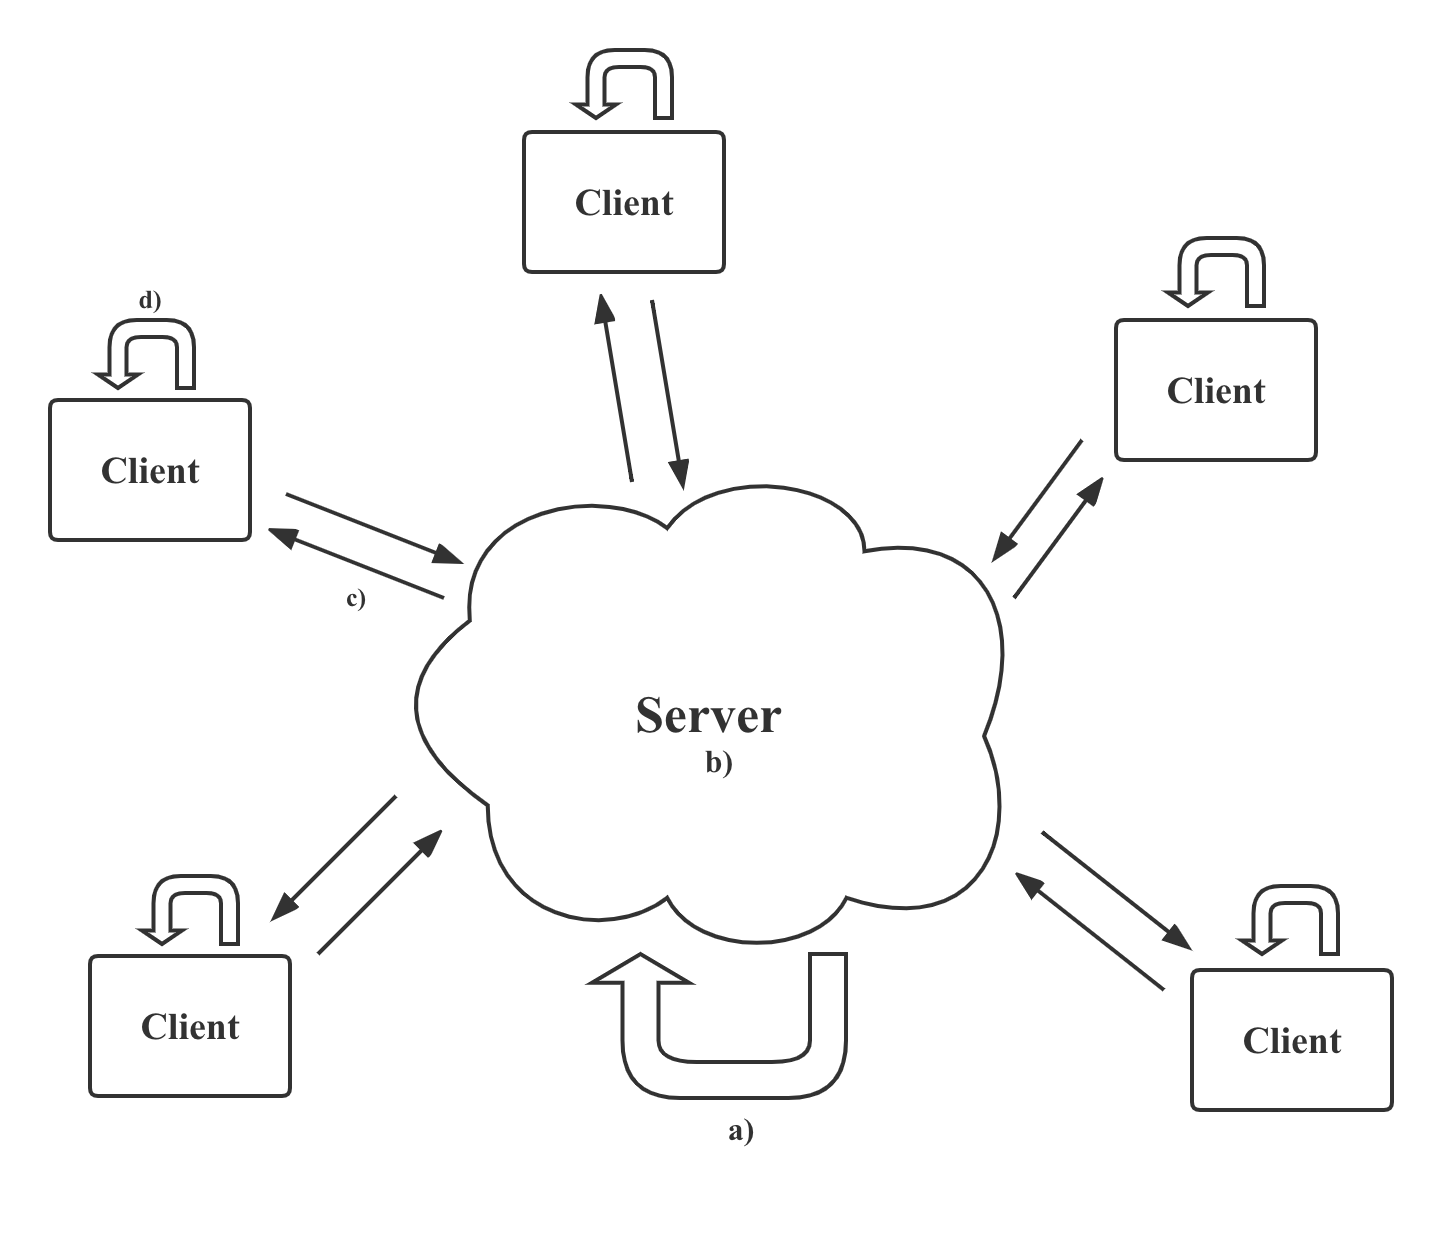
\includegraphics[width=1\textwidth]{figures/ServerClientModule.png}
    \caption{Whole Process Structure: a) Train the specified model. b) Deploy the model on the server. c) Perform the data transmitting. d) Data preprocessing, display and application of mobile segmentation models and other related tasks.}\label{ServerClientModule}
    % 图片的标题应该在下方
\end{figure}

% (移动端计算力和网络带宽/延时均有了显著提升(数据),使得在移动端部署并应用dense prediction方法成为了可能. )
And even to achieve real-time target detection on mobile terminals. The current mainstream mobile operating systems include Apple's IOS system and Android system, among which a huge amount of hardware is equipped with the Android system, which makes it have a huge user group. All mentioned above make it valuable to develop an APP with a dense prediction function on the Android end terminal.

Some traditional image segmentation algorithms such as threshold-based segmentation method \cite{al2010image}, watershed algorithm, and segmentation method based on edge detection, mostly rely on the low-level semantic information of the image to segment the image. Therefore, the segmentation results are not ideal in scenes with complex images and shredded edges. However, the paper FCN (Fully Convolutional Networks for Semantic Segmentation) \cite{long2015fully}, which was a candidate for the best paper in CVPR 2015, has greatly improved the effect of semantic segmentation using pure neural networks. FCN converts the output from a column of feature vectors to a mapped image by replacing traditional CNN's last fully connected layer with a convolutional layer. Thus, the category to which each pixel belongs is recovered from the abstract features, that is, extends from image-level classification to pixel-level classification. FCN laid the foundation for many subsequent semantic segmentation models, including FaPN \cite{huang2021fapn}, ResNet \cite{he2016deep}, etc. used in the paper.


\subsection{Research Objectives and Expected Results}
The goal of the graduation project is to reproduce the training process and results of FaPN \cite{huang2021fapn} and apply this high-accuracy dense prediction model on the mobile terminal, to realize the function of the segment and recognize objects in daily life, such as traffic signs, pedestrian, etc.

In this paper, two methods are applied and deployed on a mobile terminal to obtain better dense prediction results on the mobile terminal. The first kind uses the picture on the mobile terminal through the photo album or camera API, the verified image is then transmitted to the server end for image processing and then re-transmitted back to the front end. Another method is to apply the lightweight paddle-lite \cite{paddlelite} that has been transplanted to the mobile terminal and use the computing power of the mobile phone AI chip to process the image.

The work of paper can be mainly divided into several parts, including deploying and training the model with and without FaPN and evaluating the difference in the model accuracy, loss, AP, and mIoU to reflect the superiority of FaPN. Design an Android APP that allows users to take pictures or use existing images to identify or classify objects. Handle the interaction between the APP front-end and the server back-end. The rest of this thesis is organized as follows. 

Section \uppercase\expandafter{\romannumeral2} \textbf{Related Work}, meanly focus on introducing the main principles and functions of the related modules used and reproduced in this article. This paper gradually understands the structure and innovation of FCN, FPN, FaPN, reproduces the FSM and FAM modules of FaPN, and applies the pre-trained mobile Paddle Lite model.
%介绍本文所用到和复现的相关模块的主要原理和主要功能 本文逐渐深入地了解了FCN,FPN,FaPN的结构和创新点并复现了FaPN的FSM和FAM模块,并应用了预训练的移动端Paddle Lite模型

%主要介绍了APP服务端和客户端的开发过程和对应模块的联系和内容。包括了服务器端的模型的训练和部署,客户端网络,UI等模块的具体功能和结构。
Section \uppercase\expandafter{\romannumeral3} \textbf{FaPN Based APP}, mainly introduces the development process of the APP server and the client and the connection and content of the corresponding modules. It includes the training and deployment of the server-side module, the specific functions and structures of the client-side network, UI, and other modules. 

Section \uppercase\expandafter{\romannumeral4} \textbf{APP Results, Analysis, and Relevant Information}, analyzed training procedure and APP results. Provides information about training and running environments.


Section \uppercase\expandafter{\romannumeral4} \textbf{Conclusion and Future Work}, summarizes existing work and suggests directions for improvement.
\clearpage
% !Mode:: "TeX:UTF-8"
% !TEX program  = xelatex
\section{Related Work}
This chapter is based on the requirements of realizing image segmentation on the mobile terminal, I studied the classical FCN \cite{long2015fully} semantic segmentation algorithm and the FPN-based FaPN \cite{huang2021fapn} algorithm, analyze the problems running on the mobile terminal and choose to improve the FaPN model. After comparing MobileNet V3 and Paddle Lite \cite{paddlelite}, the Paddle Lite network was selected as the model for mobile semantic segmentation using the computing power of the mobile phone AI chip. 

% \subsection{Fully Convolutional Network}
% The FCN network structure \cite{long2015fully} was proposed by Jonathan Long et al. in 2014. Before this, the CNN network usually connects several fully connected layers after the convolutional layer and maps the feature map generated by the convolutional layer into a fixed-length feature vector. Each value of this output vector represents the probability that the input image belongs to a given class. The semantic segmentation network of the FCN network is constructed based on the convolutional neural network. The calculation in the network is the same as that in the convolution upgrade network, and there are convolutional layers, pooling layers, and activation function layers.

% Unlike classical CNNs that use fully connected layers after convolutional layers to obtain fixed-length feature vectors for classification, FCNs can accept input images of any size. FCN uses the deconvolution layer to upsample the feature map of the last convolution layer to restore it to the same size as the input image so that a prediction can be generated for each pixel while retaining the original input image. Spatial information, and finally perform pixel-wise classification on the upsampled feature map.

% The structure of the traditional CNN network is to add 4096, 4096, and 1000 channels of fully connected layers after the convolutional layer for the final predicted output. Among them, AlexNet and VGG16 are represented, which are mainly used for image classification tasks.


% \begin{figure}[htbp]
%     \centering
%     \begin{subfigure}[t]{1\linewidth}
%         \centering
%         \includegraphics[width=1\textwidth]{figures/CNN.png}
%         \caption{Typical CNN structure: usually, the CNN network will be connected to several fully connected layers after the convolutional layer, and the feature map generated by the convolutional layer will be mapped into a fixed-length feature vector. For all image-level classification and regression tasks, they expect a numerical description of the entire input image at the end. For example, AlexNet [18] outputs a 1000-dimensional vector indicating that the input image belongs to probability of which class.}\label{CNN}
%     \end{subfigure}
%     \begin{subfigure}[t]{1\linewidth}
%         \centering
%         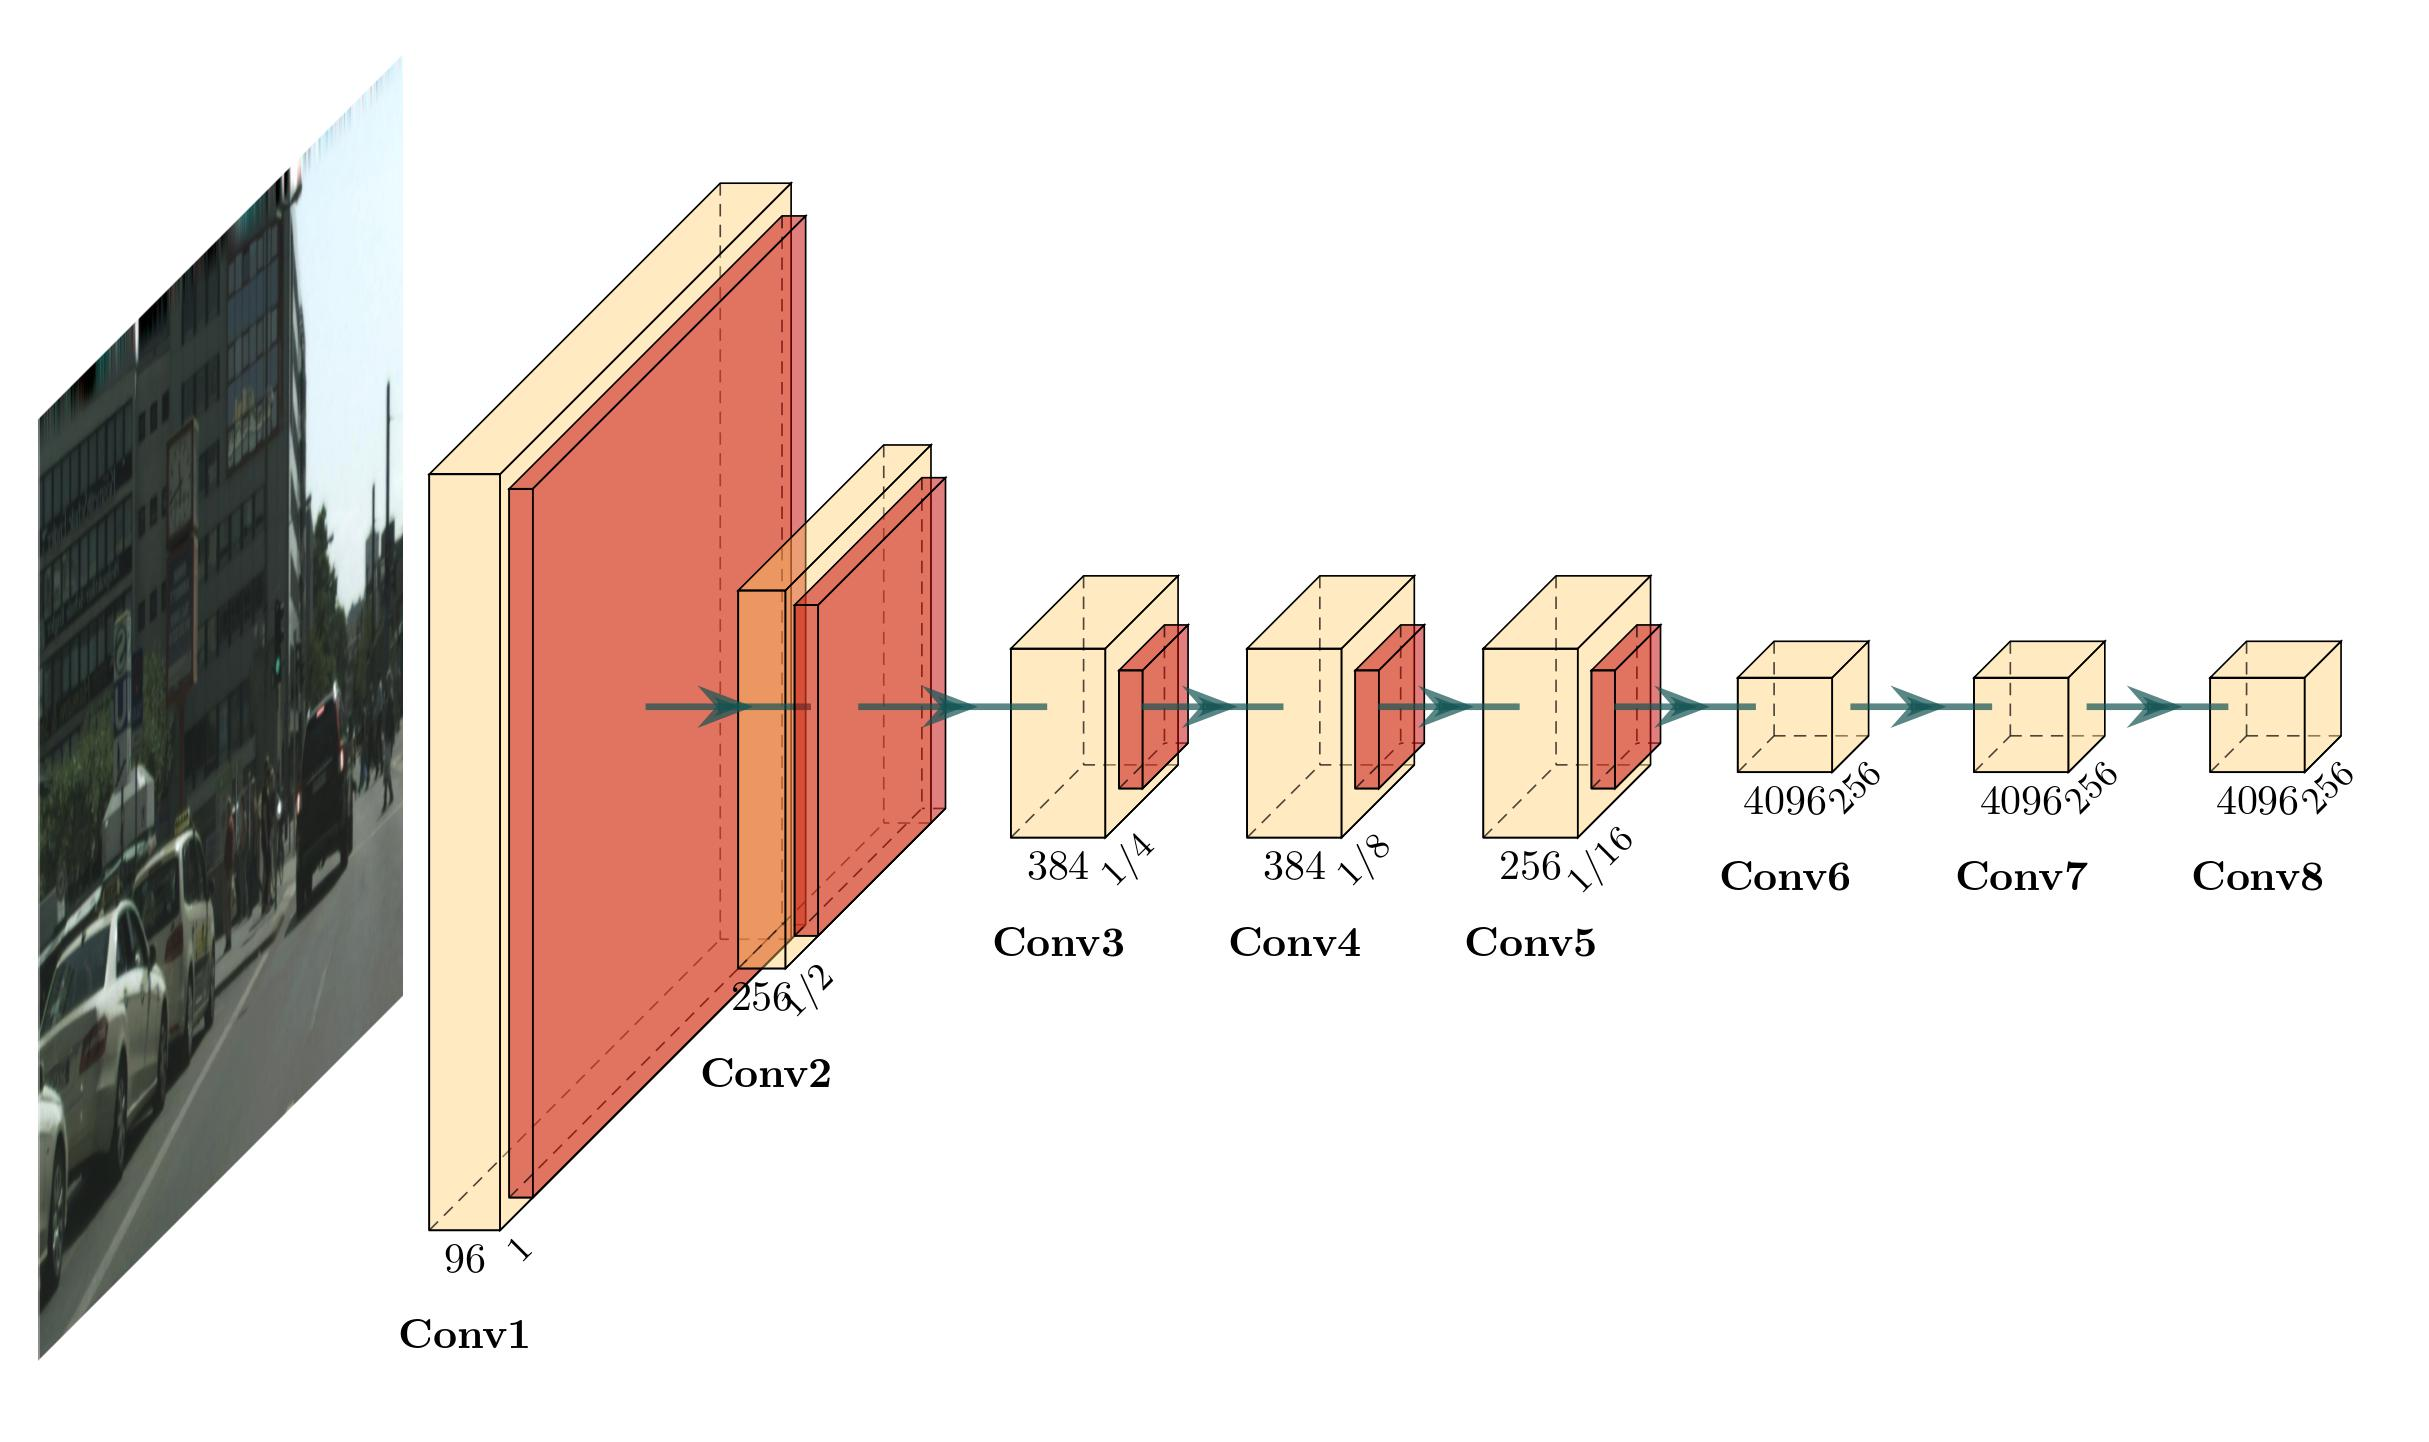
\includegraphics[width=1\textwidth]{figures/FCN.png}
%         \caption{FCN structure: FCN can accept input images of any size, and use the deconvolution layer to upsample the heat map of the last convolution layer to restore it to the same size as the input image, thus producing a prediction for every pixel.}\label{FCN}
%     \end{subfigure}
%     \caption{CNN structure compared with FCN structure}\label{FCN-CNN}
% \end{figure}


% The process of transmitting data from the bottom layer to the upper layer is called forward propagation. After the prediction result is obtained, it is compared with the ground truth, and the difference with the ground truth is obtained by calculating the loss. Then, by propagating the loss forward and updating the weight value of each layer of the network, the learning of the image is realized. This process is called backpropagation.

% % \begin{figure}[htb]
% %     \centering
% %     \includegraphics[width=1\textwidth]{figures/CNN.png}
% %     \caption{Typical CNN network structure: Usually, the CNN network will be connected to several fully connected layers after the convolutional layer, and the feature map generated by the convolutional layer will be mapped into a fixed-length feature vector. The classic CNN structure represented by AlexNet is suitable for image-level classification and regression tasks, because they all expect a numerical description (probability) of the entire input image at the end. For example, AlexNet's ImageNet model outputs a 1000-dimensional vector indicating that the input image belongs to Probability of each class (softmax normalization)}\label{CNN}
% %     % 图片的标题应该在下方
% % \end{figure}



% The FCN is not connected to the traditional fully connected layer after the convolutional layer, but a deconvolutional layer, which performs the function of upsampling and restores the obtained data to the size of the input image, to obtain a pixel-level semantic segmentation image of the original size. In the process of pooling, 1/2, 1/4, 1/8, 1/16, and 1/32 size relative to the original size image will get. 1/8, 1/16, and 1/32 images will be used for the upsampling operation. 

% Among them, 1/32 of the images mainly contain the most abstract semantic information of the original image, and thus the result obtained by direct upsampling is also the most blurred and smooth. For the same reason, upsampling results of 1/8 images are better than 1/16 images, and 1/16 images are better than 1/32 images. Because the results obtained by direct upsampling of pooling images are not ideal, the author proposes a series of upsampling networks that integrate images of various sizes, including FCN-8s, FCN-16s, FCN-32s.

% \begin{figure}[htb]
%     \centering
%     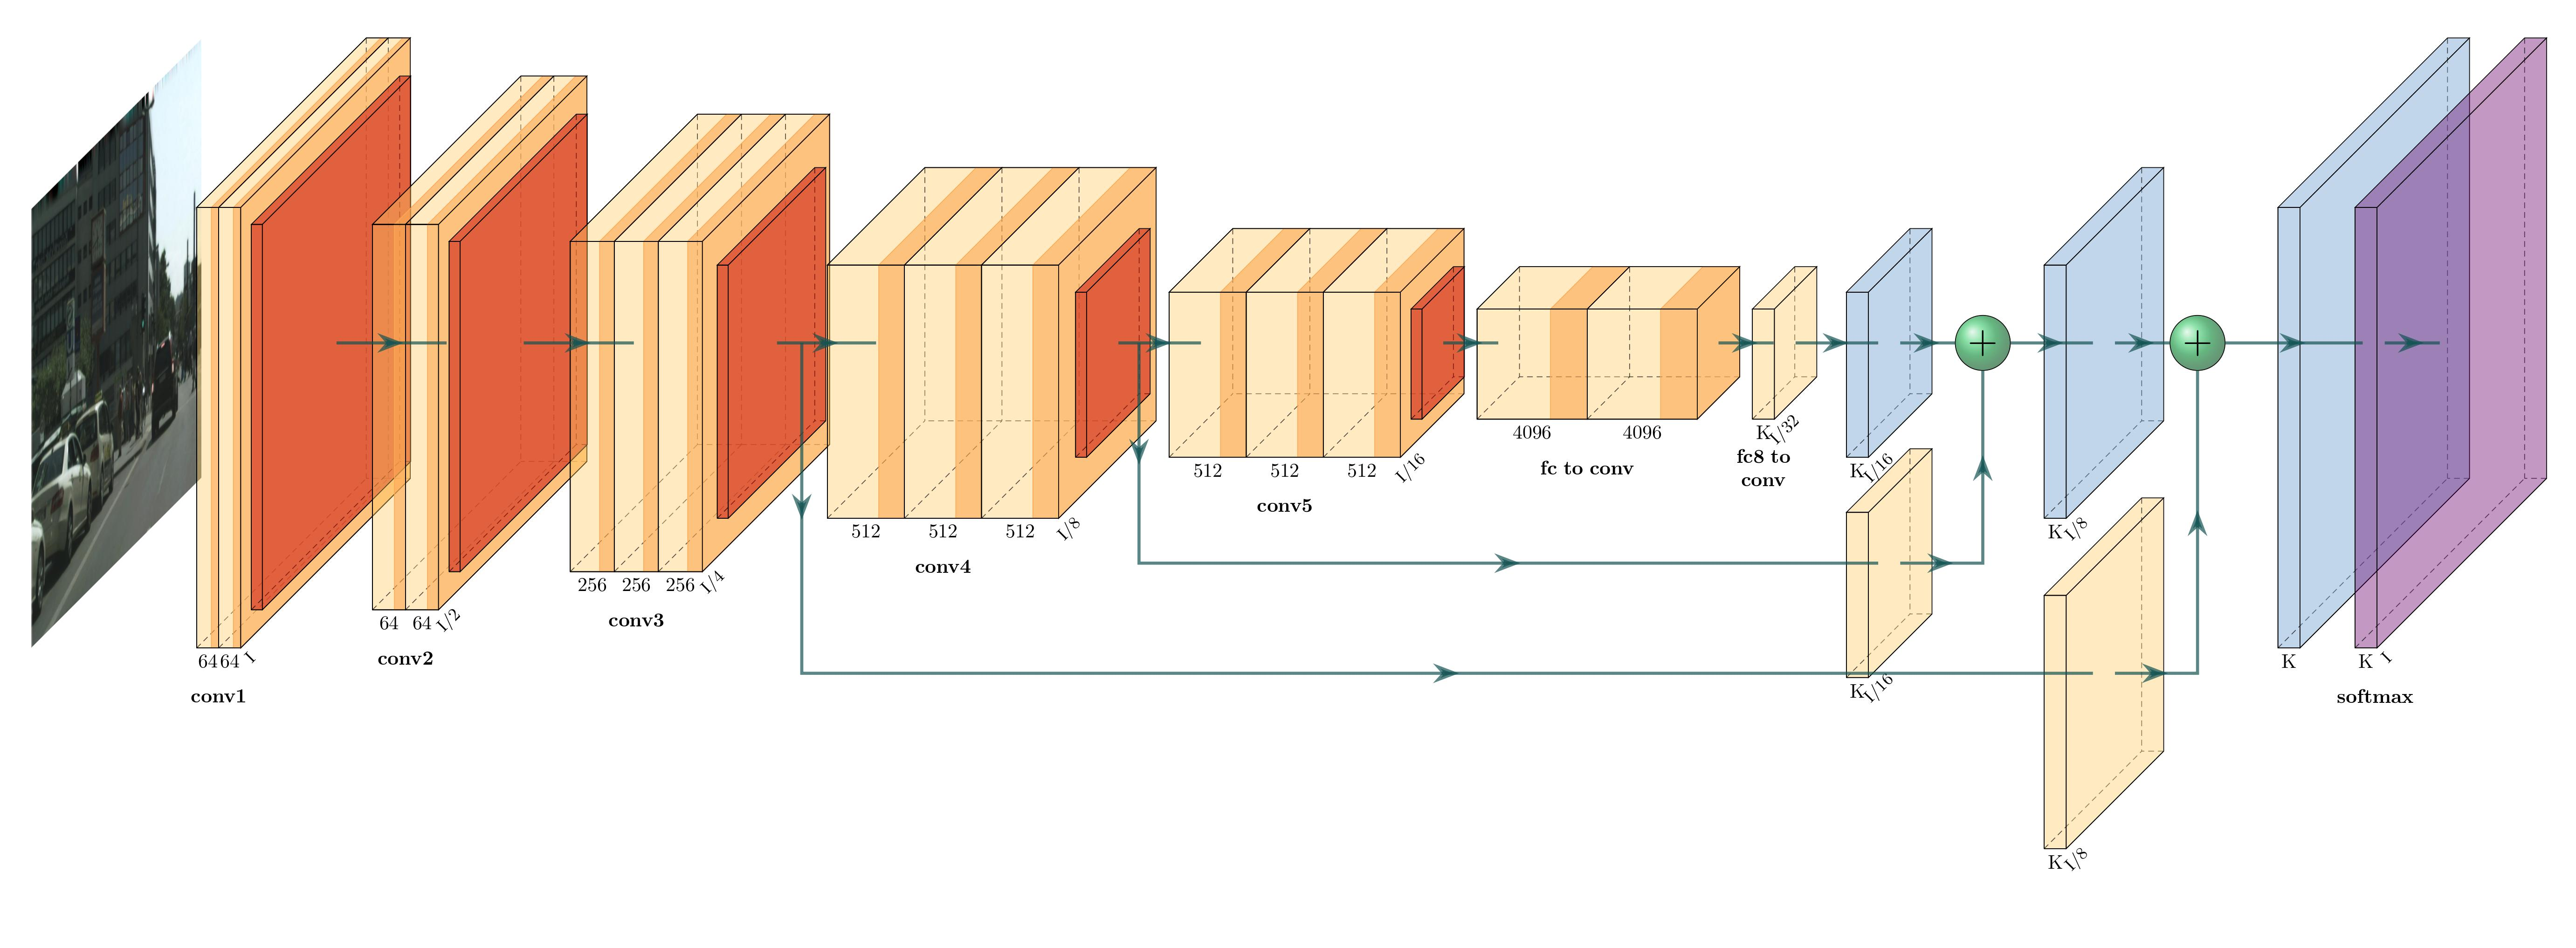
\includegraphics[width=1\textwidth]{figures/FCN8.jpg}
%     \caption{FCN-8s' Structure \cite{plotNeuralNet}}\label{FCN8}
% \end{figure}

% Among them, FCN-8s and FCN-16s use a skip-level structure to ensure the correctness of the results. By comparing the three-stage training results, FCN-8s, which utilize all levels of semantic information, have the most refined results.

% FCN innovatively uses a deconvolution layer to replace the fully connected layer and obtains pixel-level semantic segmentation results for input images of any size, and the results are better than state-of-the-art. However, the result of upsampling is not sensitive to the details of the picture, and the obtained result still has the problem of being too smooth and blurred. At the same time, the subsequently proposed ResNet50 and ResNet101 use the FCN network to improve the idea of ​​the fully connected layer and improve the effect of semantic segmentation through the residual network.

% However, compared with FPN and FaPN, FCN still has insufficient utilization of multi-level semantic information in the utilization of semantic information, and its network has many layers and a large number of parameters, so it is not suitable for porting to mobile terminals for real-time semantic segmentation.


\subsection{Feature Pyramid Networks}
Feature Pyramid Networks \cite{lin2017feature} is an article published in CVPR by Tsung-Yi Lin et al. in 2017. It integrates the semantic information of the bottom layer and the upper layer by adding a feature pyramid module to the Dense prediction problem and improves the accuracy of target detection, especially for the detection of small objects.

\begin{figure}[htbp]
    \centering
    \begin{subfigure}[t]{0.3\linewidth}
        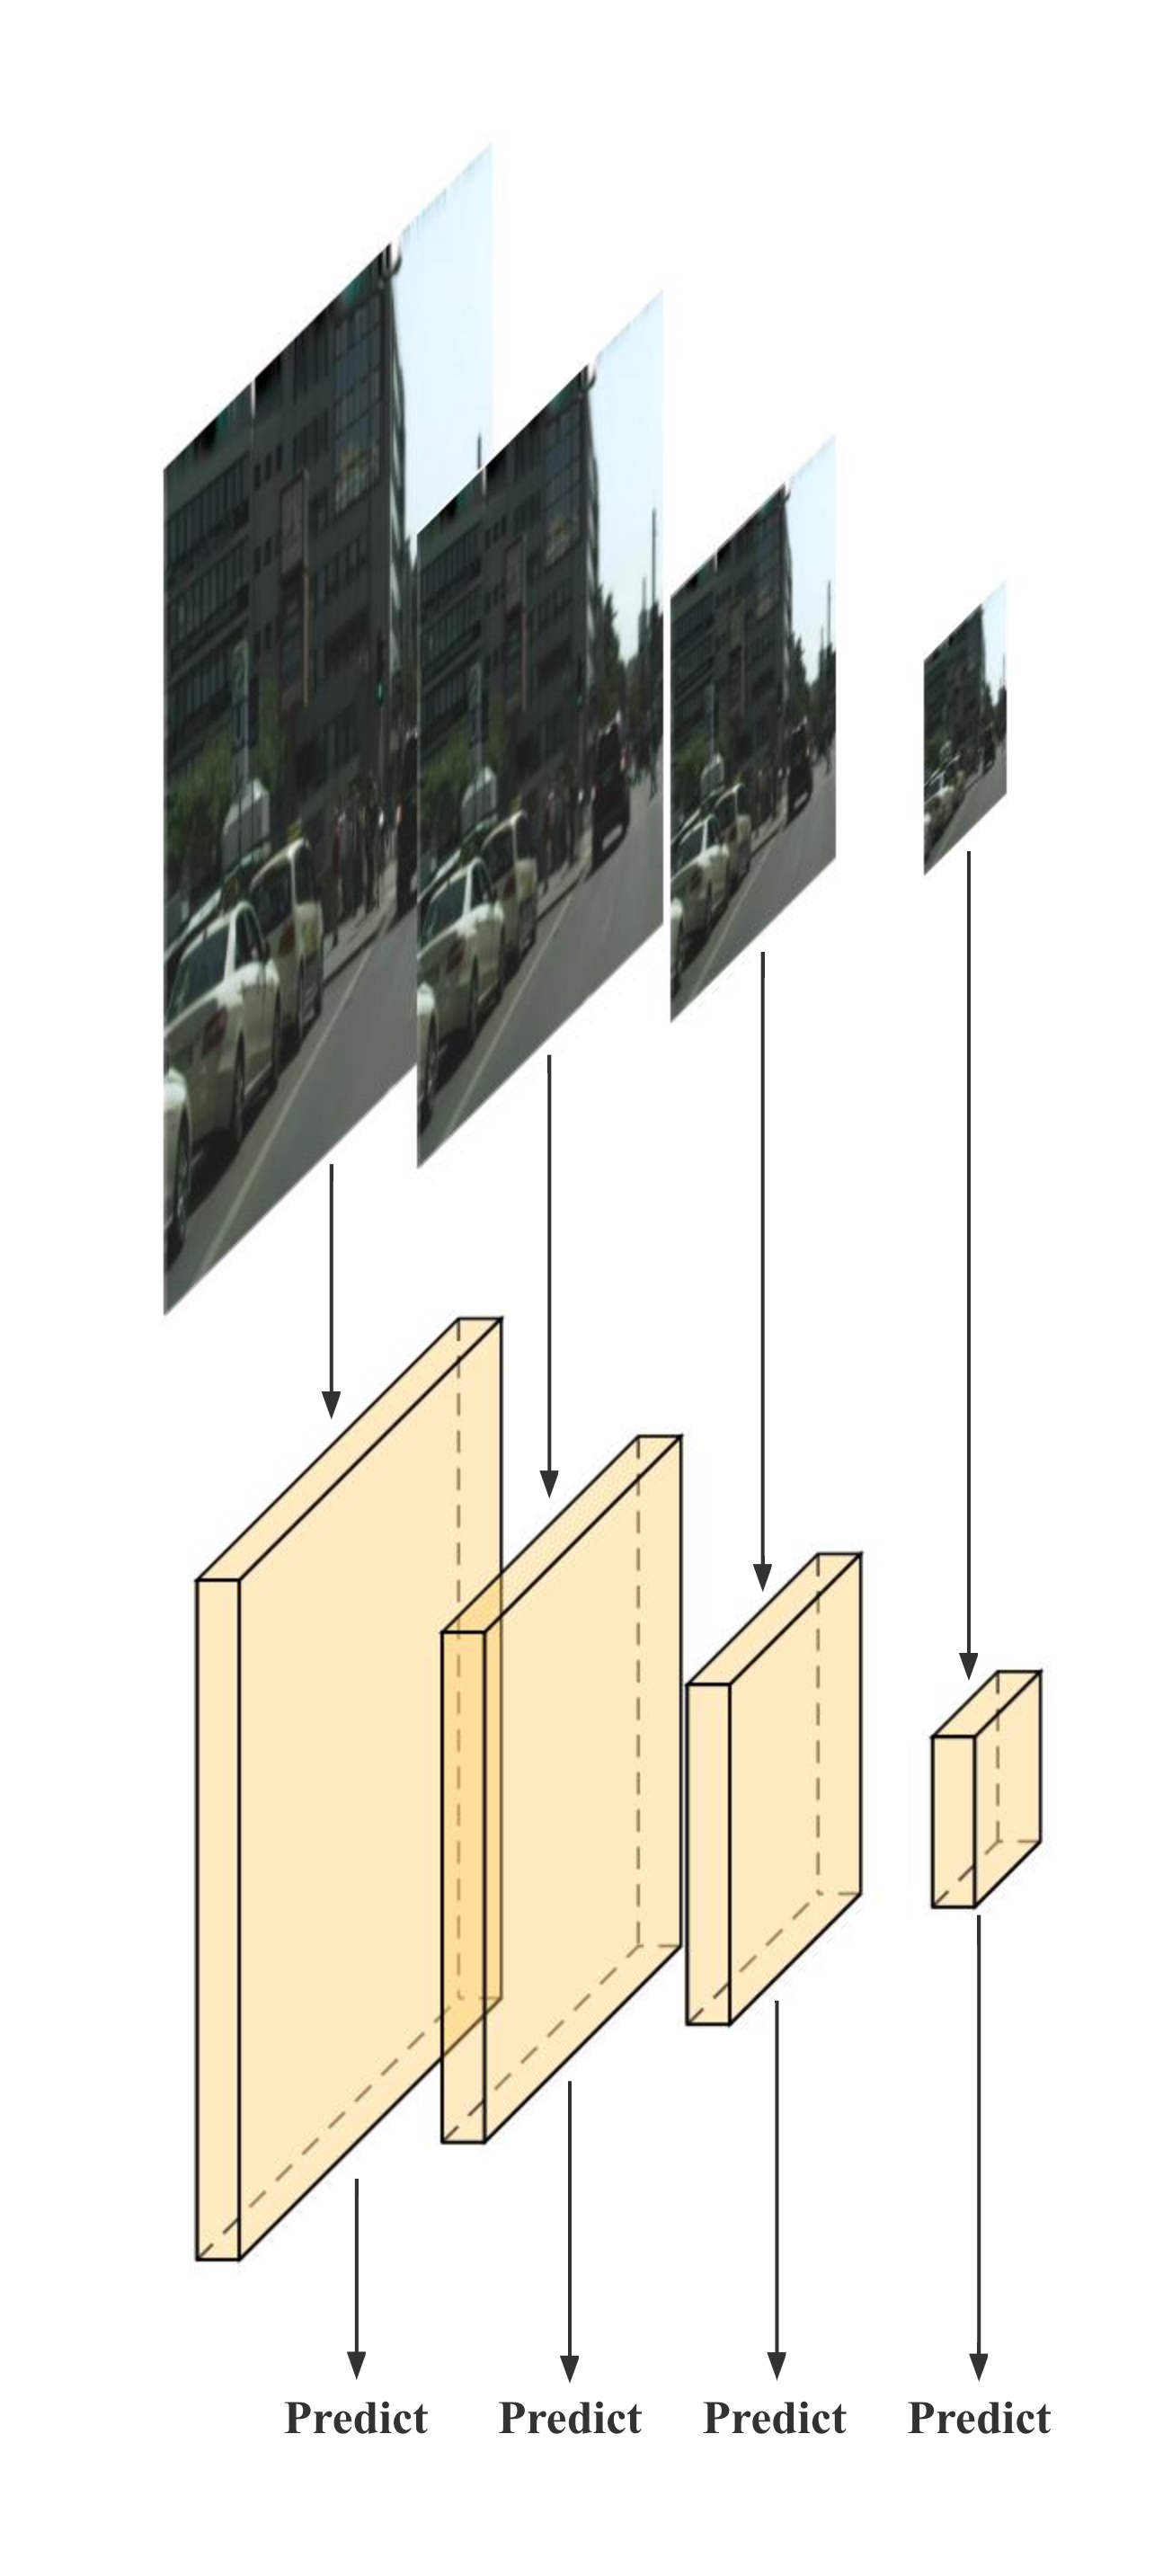
\includegraphics[width=1\textwidth]{figures/fcnarch1.png}
        \caption{Featurized Image Pyramid}\label{FCNarch1}
    \end{subfigure}
    \begin{subfigure}[t]{0.3\linewidth}
        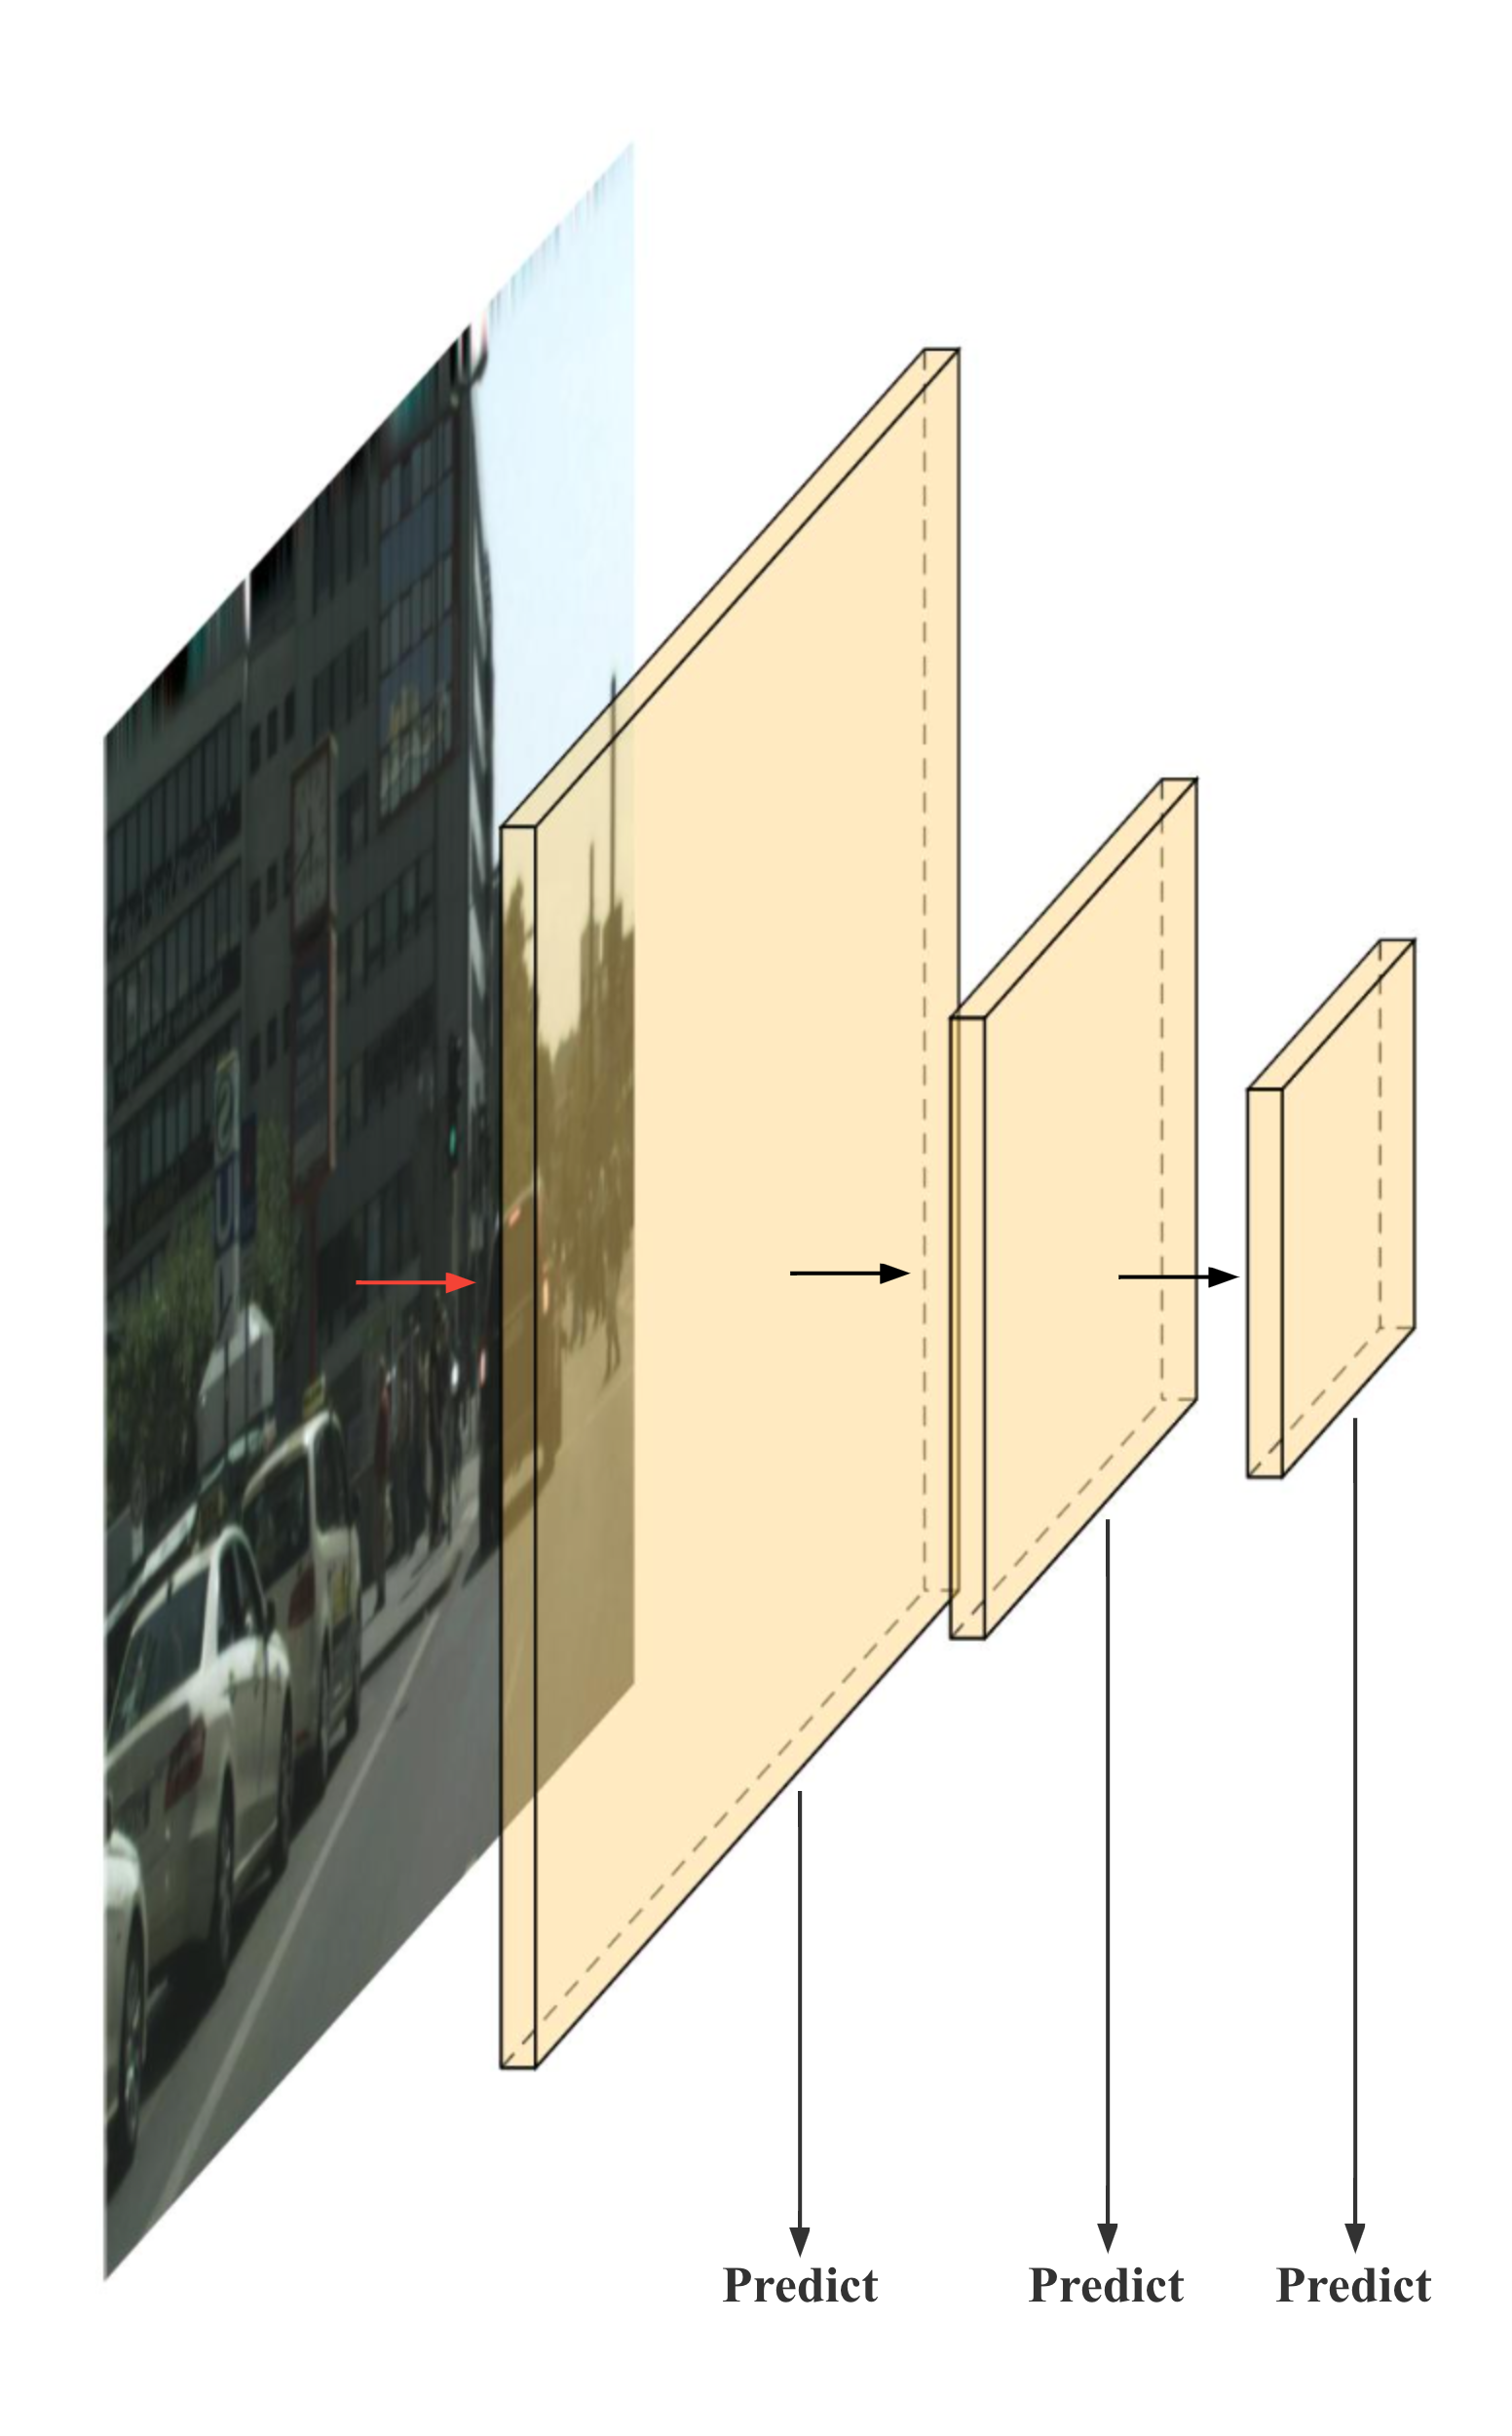
\includegraphics[width=1\textwidth]{figures/fcnarch2.png}
        \caption{Pyramid Feature Hierarchy}\label{FCNarch2}
    \end{subfigure}
    \begin{subfigure}[t]{0.3\linewidth}
        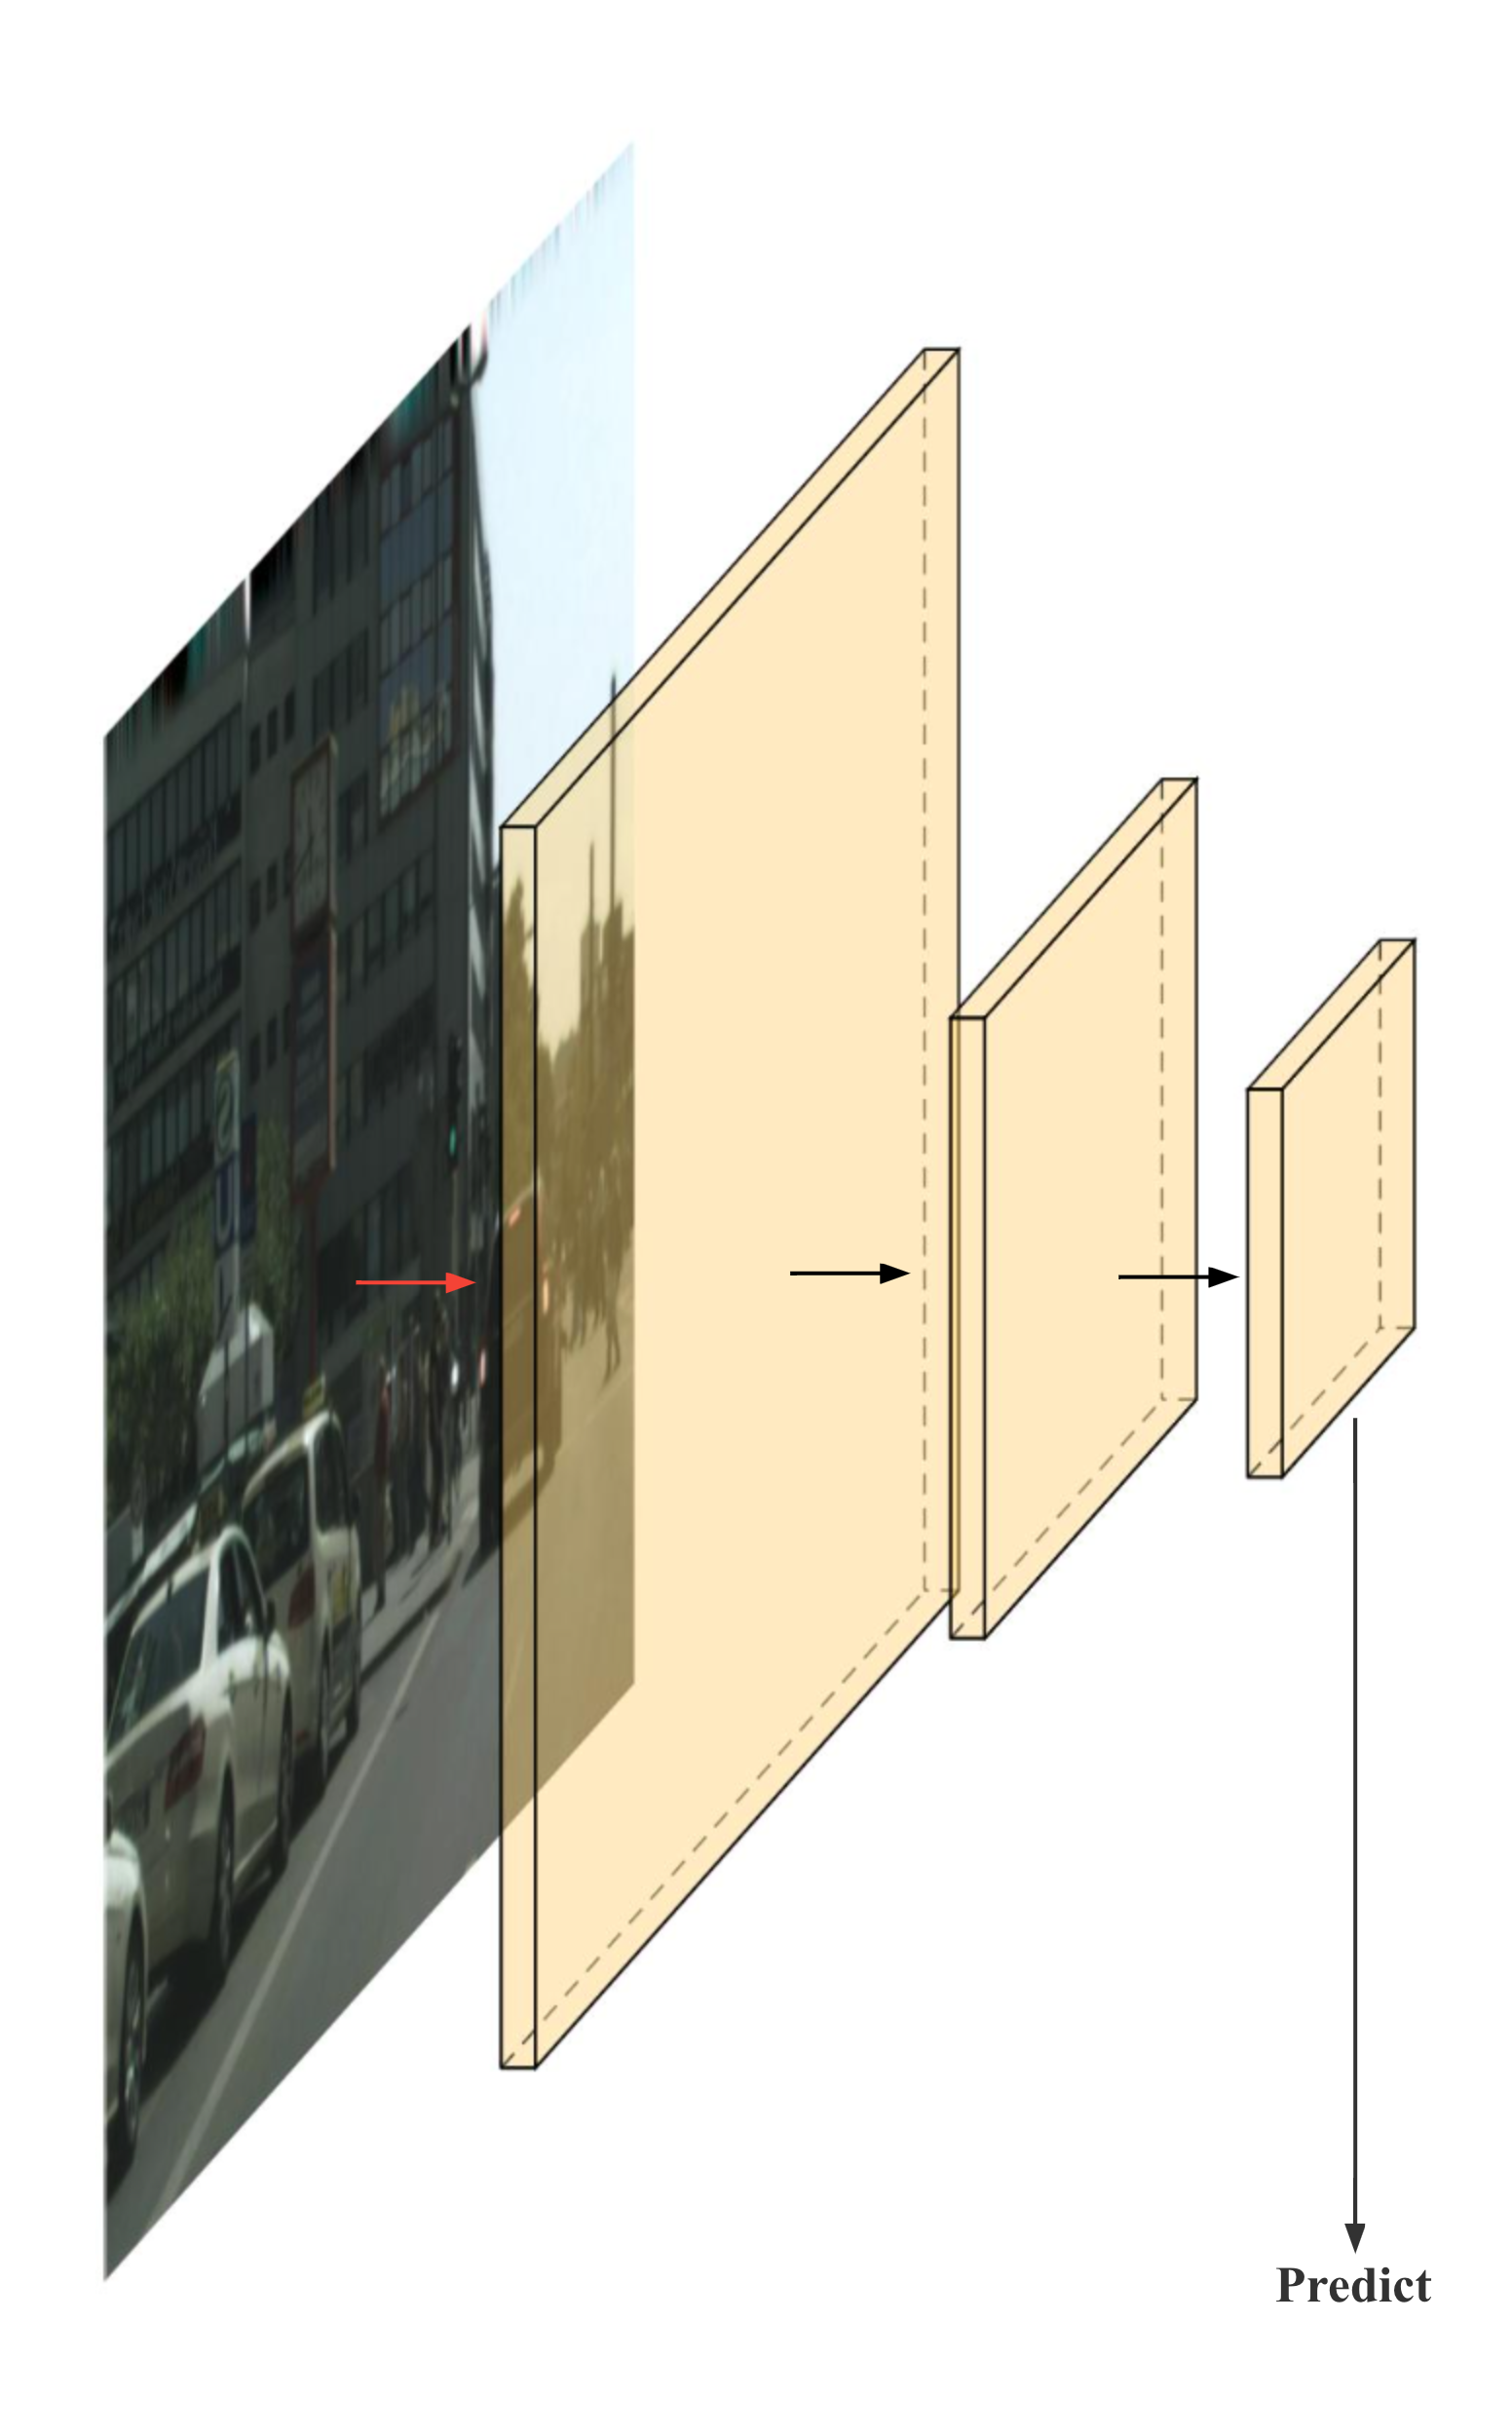
\includegraphics[width=1\textwidth]{figures/fcnarch3.png}
        \caption{Single Feature Map}\label{FCNarch3}
    \end{subfigure}
    \caption{Three typical  structures in target detection}\label{FCNarch}
\end{figure}


There are three typical structures in object detection: a) Featurized image pyramid, b) Pyramid feature hierarchy, and c) Single feature map. Among them, the Featurized image pyramid obtains the features of different scales through images of different resolutions and makes separate predictions for the features of each scale. The problem is that the time cost is too high. The pyramid feature hierarchy extracts different levels of semantic information from images through the network and predicts them separately. In this way, when high-level semantic information is used, the detection effect of small objects is not good. A single feature map only predicts the feature map of the highest layer of the network, but the resolution of the feature map of the highest layer is low, and the prediction of the position of the object is not accurate enough.

\begin{figure}[htbp]
    \centering
    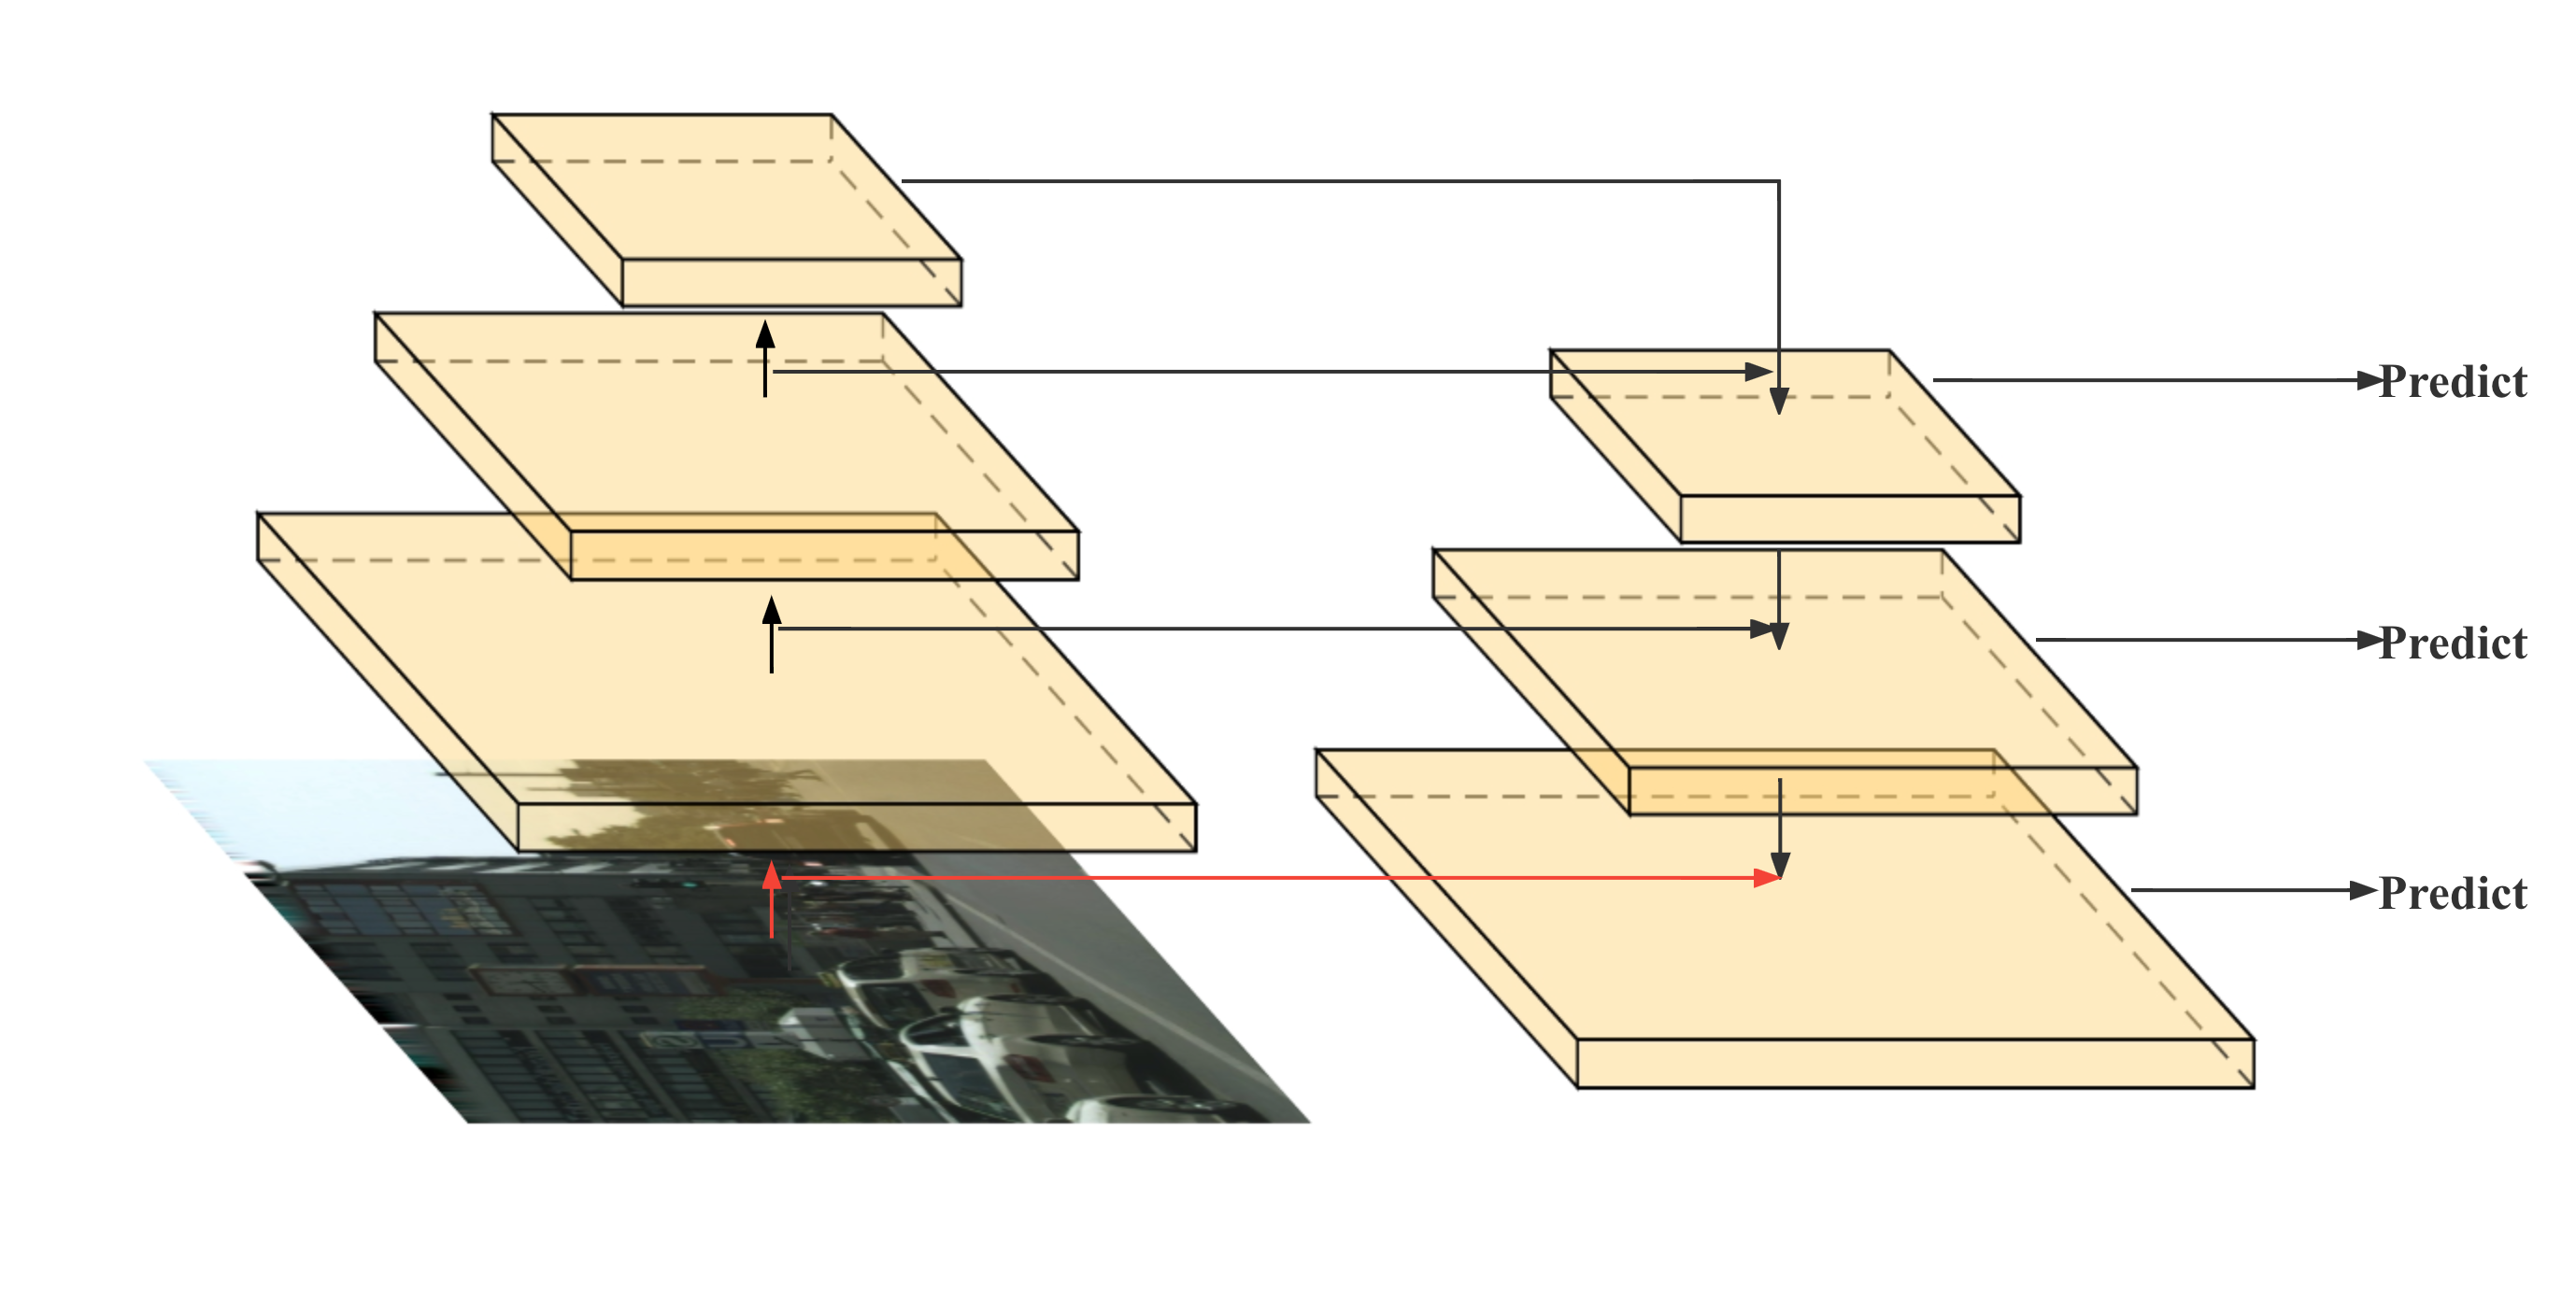
\includegraphics[width=1\textwidth]{figures/FPN_h.png}
    \caption{FPN's Structure \cite{plotNeuralNet}}\label{FPN}
\end{figure}

The FPN network uses the top-down pathway to combine the feature information of the bottom layer and the upper layer resolution. By upsampling, the more abstract high-level feature map and laterally connecting it with the lower-level feature map, the feature information of the high-level layer is strengthened. In this way, the feature information of the upper layer and the position information of the bottom layer is used at the same time, thereby improving the accuracy of dense prediction, especially for the prediction of small objects.


\subsection{Feature-aligned Pyramid Networks}

Based on FPN, Shihua Huang further proposed Feature-aligned Pyramid Networks \cite{huang2021fapn}. FPN and most of the existing networks do not consider the problem of feature alignment, which leads to the upsampling of high-level semantics, and the upsampled local features are directly filled with pixels by interpolation methods. The interpolated pixel padding can lead to misalignment of the upper and lower layer features of small objects and object boundaries, which in turn leads to misclassification in prediction.

For the above problems, the author proposes FAM (Feature Alignment Module) and FSM (Feature Selection Module) to help the model obtain more accurate upper-level semantic location information.

%两个模块解释(伪代码放在实现部分):

%因为在上卷积层向下卷积层进行上采样的过程中存在特征无法对齐的问题,所以在上采样的过程中,作者通过添加的FAM模块对这些特征样本进行了对齐。具体过程如下
Because of the problem that the features cannot be aligned in the process of upsampling the upper convolutional layer and the down convolutional layer, the author aligns these feature samples through the added FAM module during the upsampling process. The specific process is as follows:

For a given upsampled feature map $P_i$, the spatial misalignment between it and the bottom-up feature map $C_i$ is predictable.


Unaligned upsampled layers' features and bottom-up feature maps' features may lead to the wrong prediction of upsampled layers' features in the process of recursive upsampling, which in turn leads to the wrong prediction of small objects and object edges, so the alignment of features in upsampled layers' $P_i$ and bottom-up feature maps' features $C_i$ is very necessary. The spatial location information, the offset $\Delta_i$ is provided by both the feature's location in $C_i$ and $P_i$. With the information provided, the aligned feature could be calculated according to the offset $\Delta_i$ and unaligned feature $P^u_i$ in upsampled layer $P_i$. The mathematical formulation is present as in Equation (\ref{con:FAM}) \cite{huang2021fapn}

\begin{equation}
    \begin{aligned}
        \Delta_i = f_a([\hat{\textbf{C}}_{i-1}, \textbf{P}^u_i]),\\
    \hat{\textbf{P}}^u_i = f_m(\textbf{P}^u_i, \Delta_i),
    \label{con:FAM}
    \end{aligned}
\end{equation}

where $\Delta_i$ denotes the offset distance from the unaligned feature $C_i$ to the $P^u_i$, in which the $\hat{C}_{i-1}$ denotes the reference of $C_i$. $f_b(·)$ denotes the calculation procedure of the aligned feature $\hat{P}^u_i$. The algorithm is implemented by the deformable convolutions \cite{dai2017deformable}.


In the typical FPN, the bottom-up feature maps are added with the upsampled feature maps after a 1 * 1 convolutional layer. Thus, it's necessary to selectively use the useful feature. The mathematical formulation is present as in Equation(\ref{con:FSM}) \cite{huang2021fapn}

\begin{equation}
    \begin{aligned}
    \textbf{u} = f_m(\textbf{z}),\\
    \hat{\textbf{C}}_i = f_s(\textbf{C}_i+\textbf{u}*\textbf{C}_i),
    \label{con:FSM}
    \end{aligned}
\end{equation}

where the \textbf{u} indicates the importance vector, for each feature map there's an importance value to add all up. The importance value is extracted according to Equation(\ref{con:AVEPOOL}) \cite{huang2021fapn}

\begin{equation}
    \begin{aligned}
    \textbf{z}= [z_1, z_2, ..., z_D],\\
    \textbf{z}_d = \frac{1}{H_i * W_i}\sum_{h = 1}^{H_i}\sum_{w = 1}^{W_i}c_d(h,w),
    \label{con:AVEPOOL}
    \end{aligned}
\end{equation}

%这个平均池化的操作保证了对于feature map的重要特征的提取和提取后的一致性。使重要的特征得到了增强,不重要的特征被减弱。
This average pooling operation ensures the extraction and consistency of the important features of the feature map after extraction. The important features are enhanced, and the unimportant features are weakened.

% \subsection{Paddle Lite}
% Paddle Lite \cite{paddlelite} is an end-to-end reasoning engine launched by Paddle Mobile based on the new upgrade of Paddle Mobile. It is more complete in the support of multi-hardware, multi-platform and hardware hybrid scheduling, and provides efficient and lightweight AI applications for end-side scenarios including mobile phones. Reasoning ability, effectively solve problems such as mobile phone computing power and memory limitations, and are committed to promoting the wider implementation of AI applications.

\clearpage
% !Mode:: "TeX:UTF-8"
% !TEX program  = xelatex

\section{Construction}




\subsection{Jetson Nano环境搭建}
待完成

\subsection{Model Training}

%此部分主要介绍了在不同的数据集上使用不同的backbone网络+FaPN进行训练,并评估了在数据集的测试集上的性能。

In this section, I mainly introduce the training process of different backbone networks with FaPN on different datasets and evaluates the performance on the test set of the dataset.

\textbf{COCO 2017 Dataset: }MS COCO \cite{lin2014microsoft} consists of over 100K images with different objects and annotations including bounding boxes and segmentation masks. I use the train2017 set (about 118K images) for training and report the results val2017 set (5K images) for comparison. For both object detection and instance segmentation tasks, there are 80 categories; for panoptic segmentation tasks, there are 80 stuff and 53 stuff classes annotated.


\begin{table}[htb]
	% h-here,t-top,b-bottom,优先级依次下降
		\begin{center}
		% 居中
			\caption{Notations}\label{Notation}
			\begin{tabular}{|c|l|} % 三线表不能有竖线,l-left,c-center,r-right
				\toprule
				\textbf{Notation} & \textbf{Definition}\\
				\hline
				$f_a(·)$ & feature aligned procedure\\
				$f_s(·)$ & feature selection procedure\\
				$f_m(·)$ & feature importance modeling procedure\\
				$P^u_i$ & unaligned feature i in upsampled layer\\
				$\textbf{z}$ & importance value set\\
				$\Delta_i$ & offset distance\\
				$C_i$ & unaligned feature i\\
				$H$ & height of the feature map\\
				$W$ & width of the feature map\\
				$x_\textbf{p}$ & feature in the given position p\\
				$\Delta\textbf{p}_n$&tuple of the additional offset\\
				$f_i$&aligned feature i\\
				$AP$&average precision\\
				\bottomrule
			\end{tabular}
		\end{center}
	\end{table}

The deformable convolution is used in the feature aligned procedure. It can be mathematically presented as Equation(\ref{con:deformableConvolution}).



\begin{equation}
    \begin{aligned}
    \hat{x}_\textbf{p}= \sum_{n = 1}^{N}w_n * x_{\textbf{p}+\textbf{p}_n},
    \label{con:deformableConvolution}
    \end{aligned}
\end{equation}

input $\textbf{c}_i \in \mathbb{R}^{H_i * W_i}$ is the feature map and the conv layer with $k * k$. The output $\hat{x}_\textbf{p}$ is the feature in the given position $\textbf{p}$. Then it can be calculated according to the sum of the convolution procedure. However, for the FAM module, the additional offset distance is added, so the Equation(4) can be reformulated as Equation(\ref{con:famConvolution}).

\begin{equation}
    \begin{aligned}
    \hat{x}_\textbf{p}= \sum_{n = 1}^{N}w_n * x_{\textbf{p}+\textbf{p}_n+\Delta\textbf{p}_n},
    \label{con:famConvolution}
    \end{aligned}
\end{equation}

where the $\Delta\textbf{p}_n$ is a tuple $[h, w] \in [(-H_i, H_i), (-W_i, W_i)]$.

\begin{algorithm}[htbp]
	\caption{Pseudo-Code of Feature Aligned Module} 
	\label{alg1} 
	\begin{algorithmic}
		\REQUIRE 
        The input channel, $C_{in}$;
		\ The output channel, $C_{out}$;
		\ The bottom-up feature map, $f_m$;
		\ The top-down feature map, $f_t$;
		\ENSURE 
        The aligned feature, $\hat{f}_i$;
		\STATE Execute the FSM module with $C_{in}$ and $C_{out}$.
		\STATE Initialize the offset layer with nn.Conv2d.
		\STATE Use nn.Relu as the activation function.
		\IF{$f_m$'s size not equals to the size of $f_t$}
        \STATE Use F.interpolate to upsample the $f_t$.
		\ENDIF 
		\STATE Select important features $\hat{f}_t$ through FSM module.
		\STATE $\hat{f}_i \gets \hat{f}_t + f_m$.

	\end{algorithmic} 
\end{algorithm}

\begin{algorithm}[htbp]
	\caption{Pseudo-Code of Feature Selection Module} 
	\label{alg2} 
	\begin{algorithmic}
		\REQUIRE 
        The input channel, $C_{in}$;
		\ The output channel, $C_{out}$;
		\ENSURE The selected feature, $\hat{f}_i$;
		\STATE Use F.avg\_pool2d to get the result of average pool of input feature map.
		\STATE Use nn.Conv2d to get the feature vector $\textbf{z} =  [z_1, z_2, ..., z_D]$.
		\STATE Multiply the $\textbf{z}$ with input feature map, get the result $x$.
		\STATE $C_{out} \gets nn.Conv2d(C_{in}, C_{out}, 1, x)$. 

	\end{algorithmic} 
\end{algorithm}


FaPN adds feature selection module \cite{hu2018squeeze} and feature aligned module based on FPN. Compared with FPN, Instance Segmentation has achieved 1.2\%-2.6\% improvement \cite{huang2021fapn}. The FaPN-based modules in this paper are all trained on the COCO2017 dataset in the aforementioned backbone networks. The training parameters are presented in the relevant environment for the training and running section.


For the performance evaluation of the above-mentioned models, Average Precision, that is, the AP value is the main evaluation index. The AP value can be divided into $AP_s$, $AP_m$, and $AP_l$ according to the size of the detection target; $AP_s$, $AP_m$, and $AP_l$ respectively represent small, medium and large The detection effect of objects. mIoU, also known as mean Intersection-over-Union, is mainly used to evaluate the performance of semantic segmentation \cite{padilla2021comparative}.

%miou,两框交集/两框并集
$$ mIoU = \frac{1}{k+1} \sum_{i=0}^{k}\frac{p_{ii}}{\sum_{i=0}^{k}p_{ij}+\sum_{j=0}^{k}p_{ji}-p_{ii}}$$

$$AP = \frac{1}{N}\sum_{n=1}^{N}Pr_{interp}(R_r(n))\ $$
$$AP_s = AP (small\ objects\ that\ area < 32^2)$$
$$AP_m = AP (medium\ objects\ that\ 32^2 < area < 96^2)$$
$$AP_l = AP (large\ objects\ that\ area > 96^2)$$

\begin{figure}[htb]
    \centering
    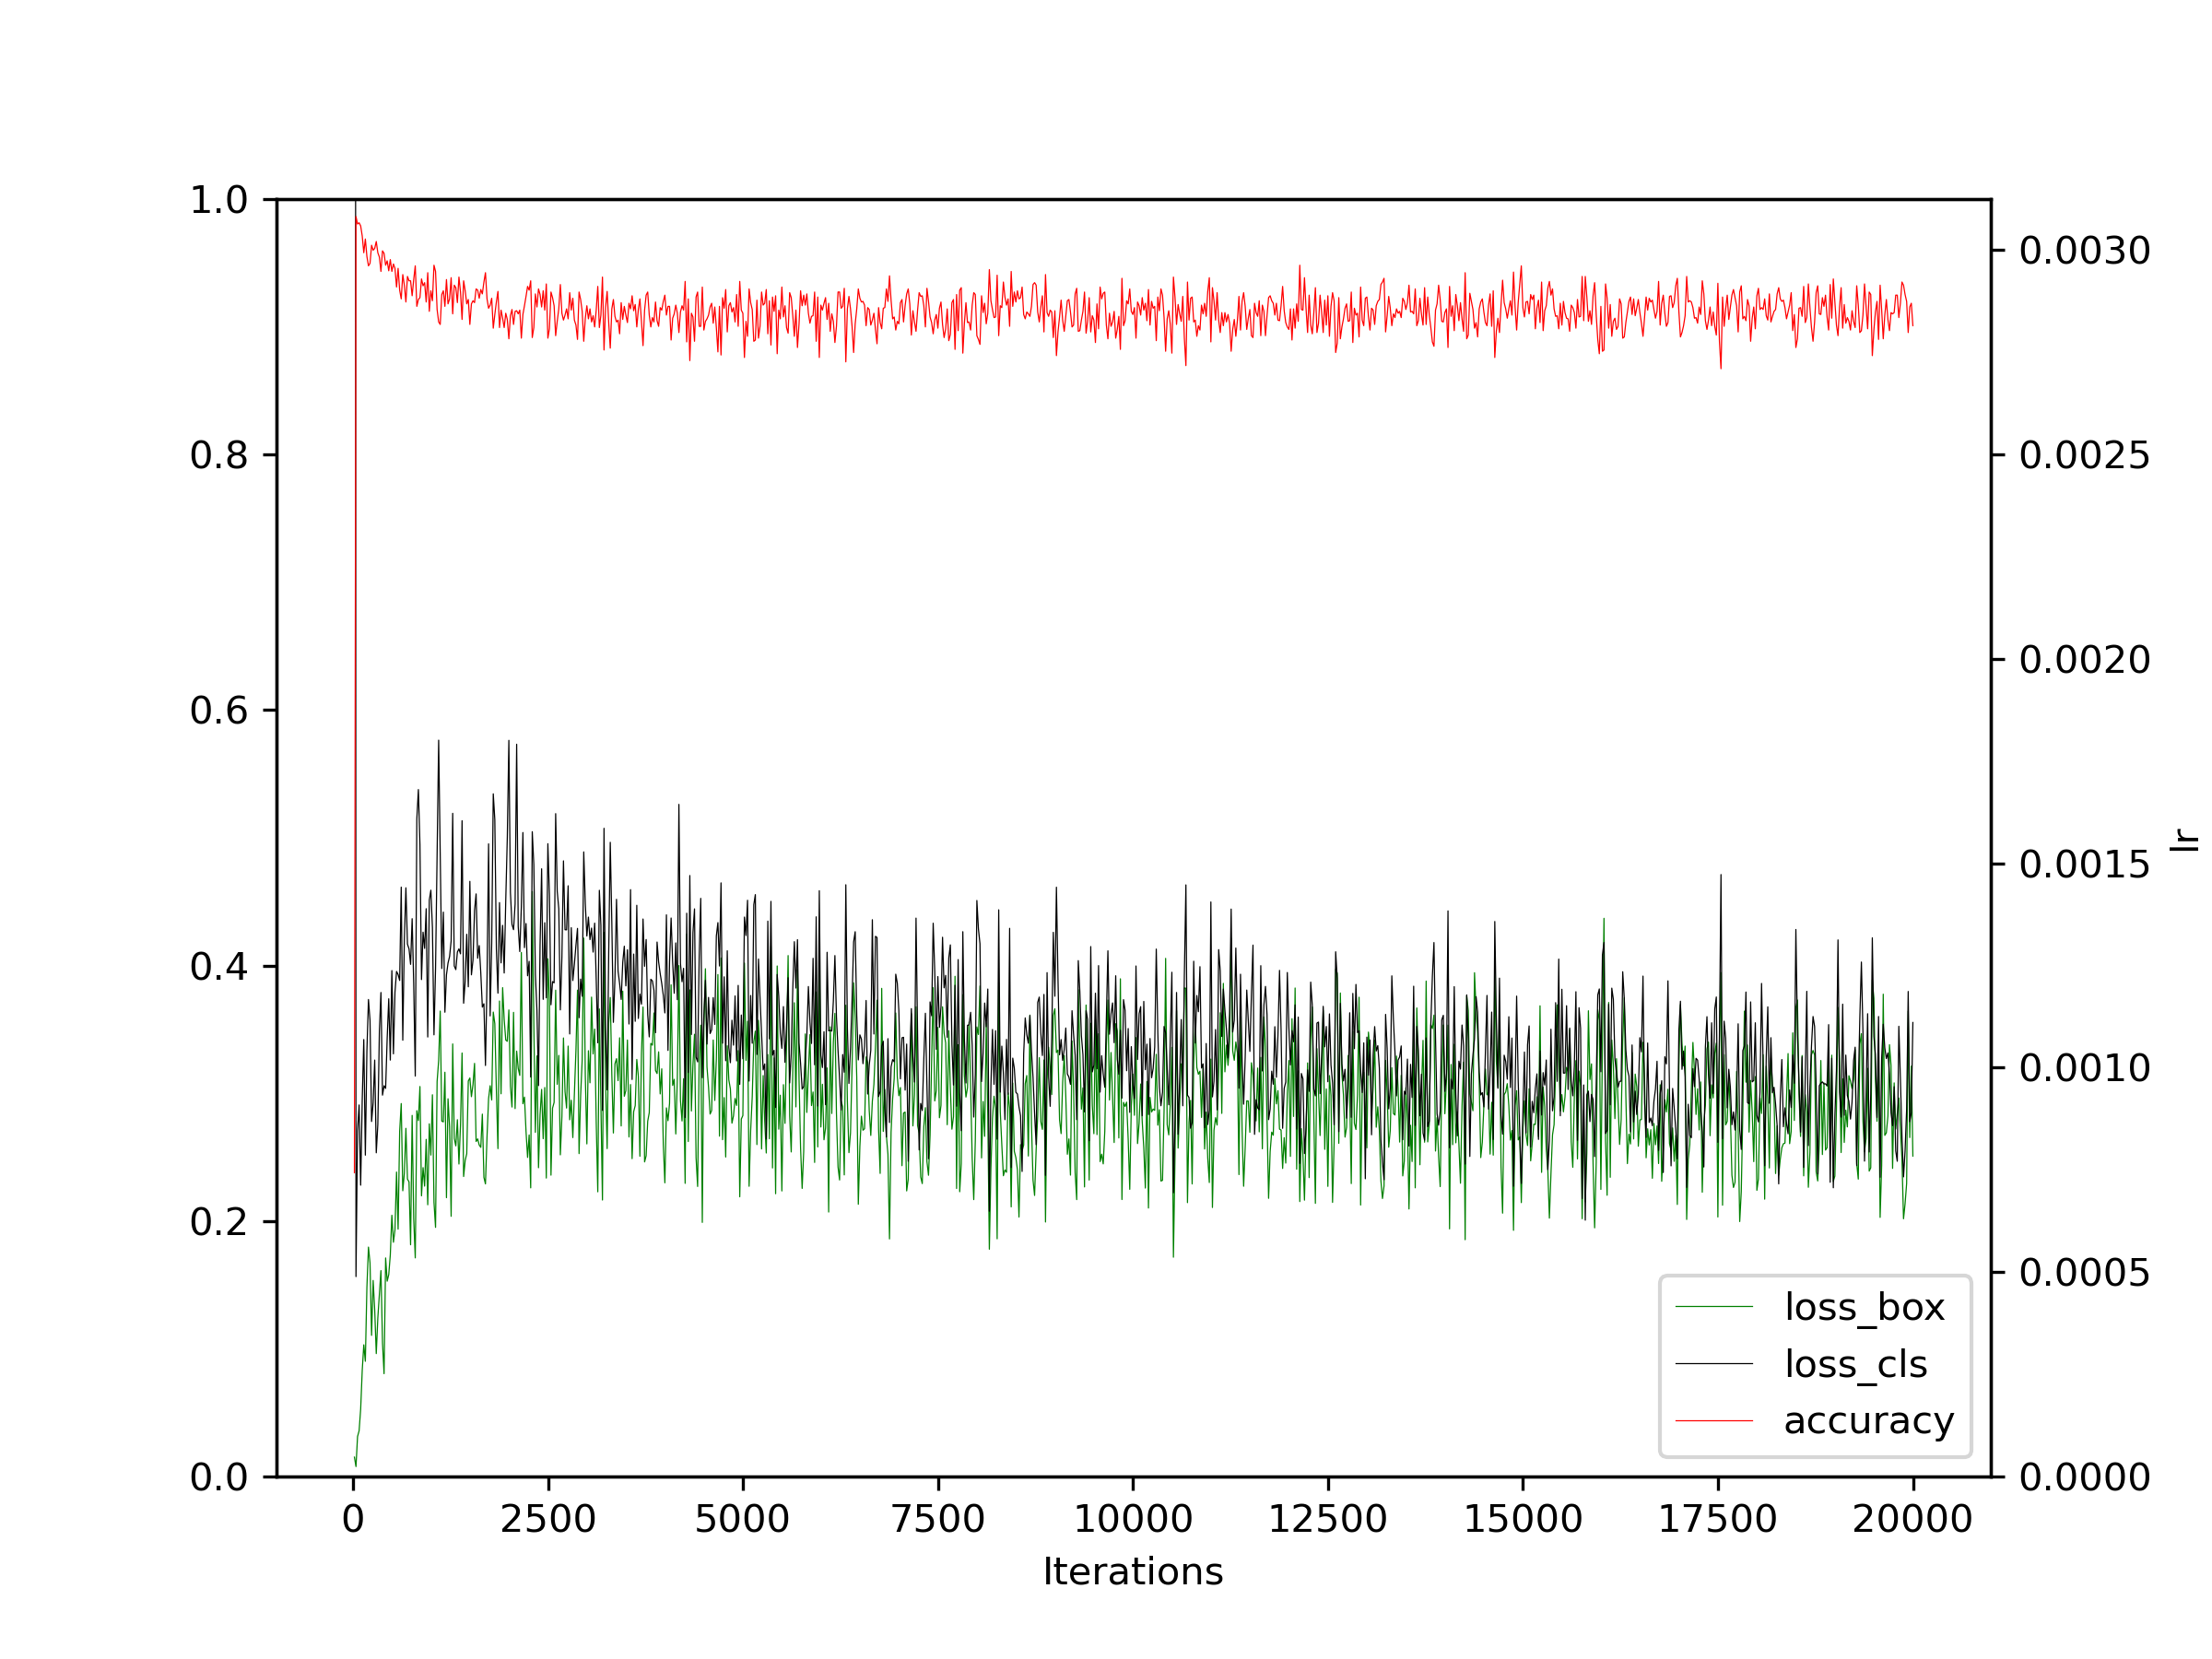
\includegraphics[width=1\textwidth]{figures/mask_rcnn_r_50_fapn_1x_20000iter.png}
    \caption{Mask RCNN \& FaPN with 20000 interactions}\label{mask_rcnn_r_50_fapn_1x_20000iter}
\end{figure}


It can be seen that after 20000 iterations and default parameter training, the accuracy rate has stabilized at the level of 95\%, and both loss box and loss cls are proficient to within 0.002, with sufficient performance for use.


Then Faster RCNN \cite{ren2015faster} was trained on 10,000 iterations after adding the FaPN module, and the results shown in the figure below were obtained.

% \begin{figure}[htb]
%     \centering
%     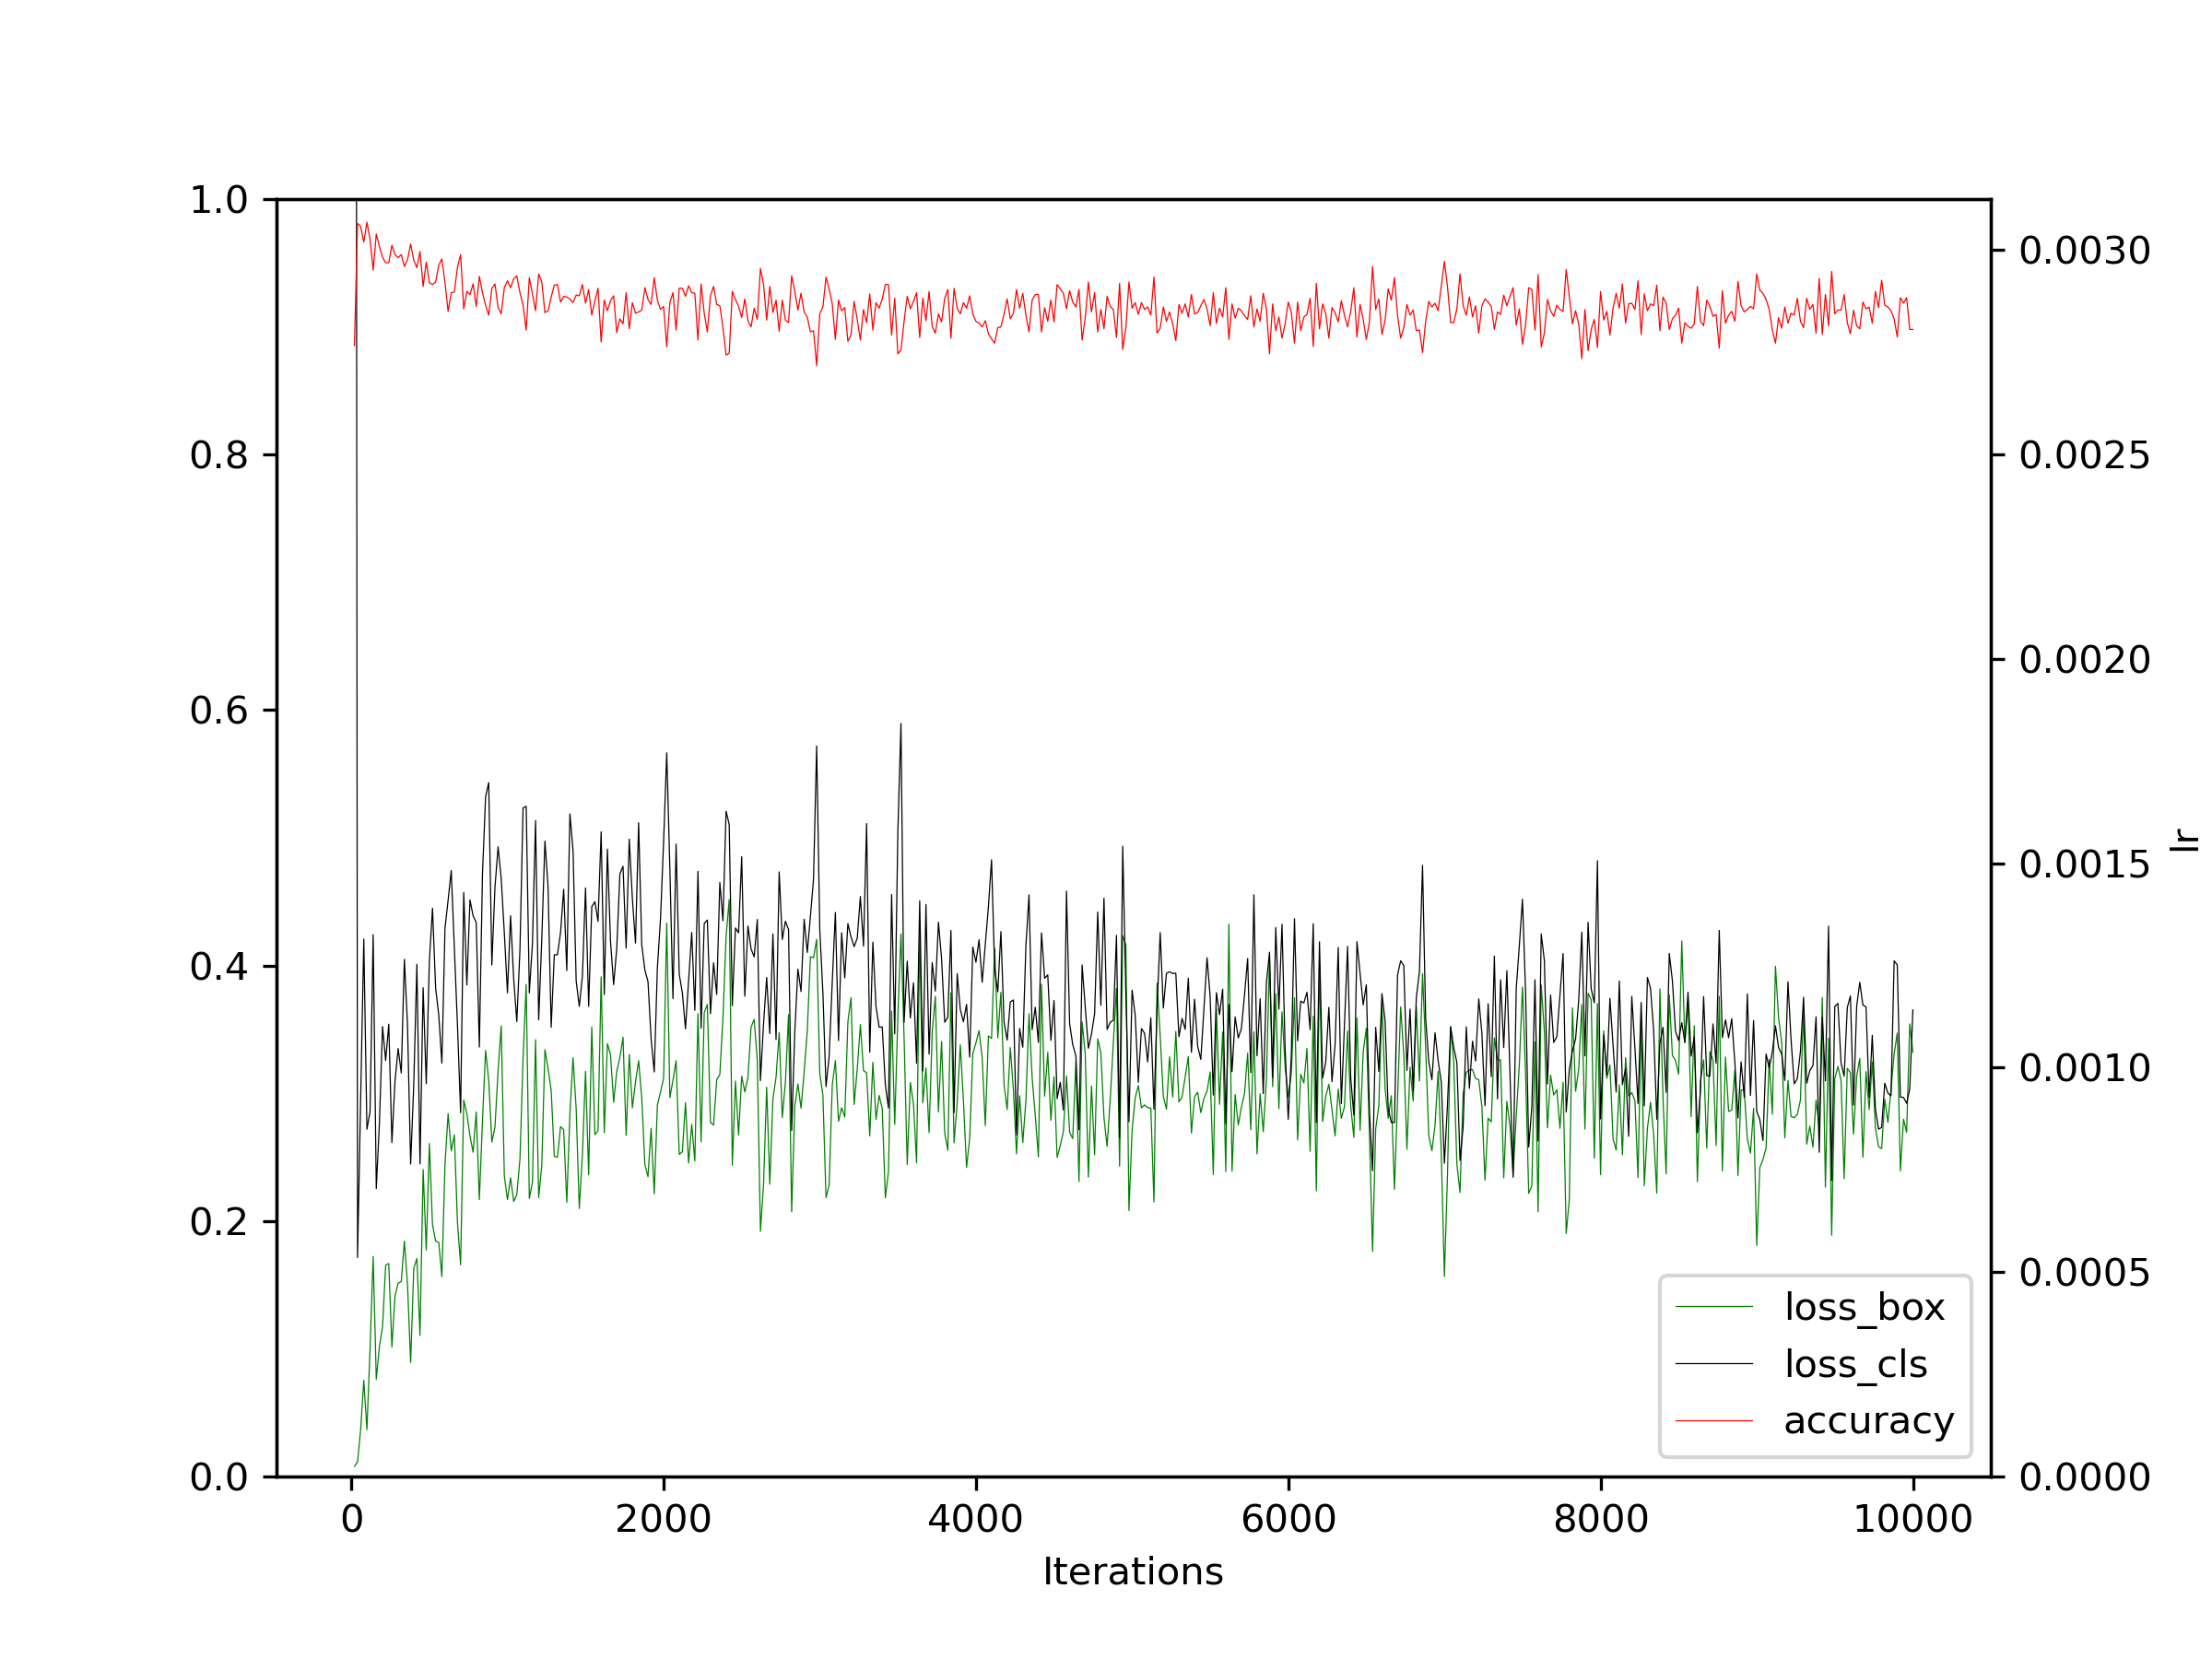
\includegraphics[width=1\textwidth]{figures/faster_rcnn_r_50_fapn_1x_10000iter.png}
%     \caption{Faster RCNN \& FaPN with 10000 interactions}\label{faster_rcnn_r_50_fapn_1x_10000iter}
% \end{figure}


It can be seen that whether Mask RCNN \cite{he2017mask} or Faster RCNN plus FaPN is used for training on the COCO2017 dataset, higher accuracy and better performance can be obtained under 10,000 iterations, and it has strong practicability.


\begin{table}[htb]
% h-here,t-top,b-bottom,优先级依次下降
    \begin{center}
    % 居中
        \caption{Performance of the Faster RCNN on category pedestrian}\label{table1}
        \begin{tabular}{|c|c|c|c|c|c|c|} % 三线表不能有竖线,l-left,c-center,r-right
            \toprule
            %三线表-top 线
            \textbf{Method} & \textbf{Backbone}&\textbf{Iterations} & $AP$ & $AP_s$ & $AP_m$ & $AP_l$ \\
            \hline
            %三线表-middle 线
            FaPN          & \multirow{5}{*}{Faster R-CNN R50}&10K &10.1&5.3&11.4&11.9 \\
            FaPN          &  &20K&12.6&9.5&12.8&15.7 \\
			FaPN (fully trained)         & &65K &40.2&23.9&43.9&48.8 \\
			FaPN (authors')         &  &-&39.2&24.5&43.3&49.1 \\
			FPN  & &- &37.9&22.4&41.1&49.1 \\
            \bottomrule
            %三线表-底线
        \end{tabular}
    \end{center}
\end{table}

\begin{table}[htb]
	% h-here,t-top,b-bottom,优先级依次下降
		\begin{center}
		% 居中
			\caption{Performance of the Mask RCNN on category pedestrian}\label{table2}
			\begin{tabular}{|c|c|c|c|c|c} % 三线表不能有竖线,l-left,c-center,r-right
				\toprule
				%三线表-top 线
				\textbf{Method} & \textbf{Backbone}&\textbf{Iterations} & $AP^{mask}$ & $AP^{mask}_s$ \\
				\hline
				%三线表-middle 线
				FaPN & \multirow{5}{*}{Mask R-CNN R50}&10K&9.5&4.0 \\
				FaPN & &20K&14.4&5.9 \\
				FaPN (fully trained) & &80K &37.2&18.3 \\
				FaPN (authors') & &- &36.4&18.1 \\
				FPN & &- &35.2&17.1 \\
				\bottomrule
				%三线表-底线
			\end{tabular}
		\end{center}
	\end{table}


\subsection{Model Deployment}


For a trained model, we can get its checkpoint (.pth) file, which holds all the parameters of the model. If we need to deploy or evaluate a trained model, we only need to use the checkpoint file of the corresponding model.


For the server-side, we need a communication module. The function of this module is to receive the front-end data and complete the processing, call the corresponding model to complete the semantic segmentation of the image, and finally return the segmented image to the client.


The server-side adopts the socket server framework, and its basic idea is to monitor the specified port of the server. After receiving the connection request from the client, it makes a handshake with it to establish a connection. Then receive and process the relevant information and call the model.




\clearpage
\section{Results, Analysis, and Relevant Information}

图片待改

\subsection{Results and Analysis}
\begin{figure}[htbp]
    \centering
    \begin{subfigure}[t]{0.4\linewidth}
        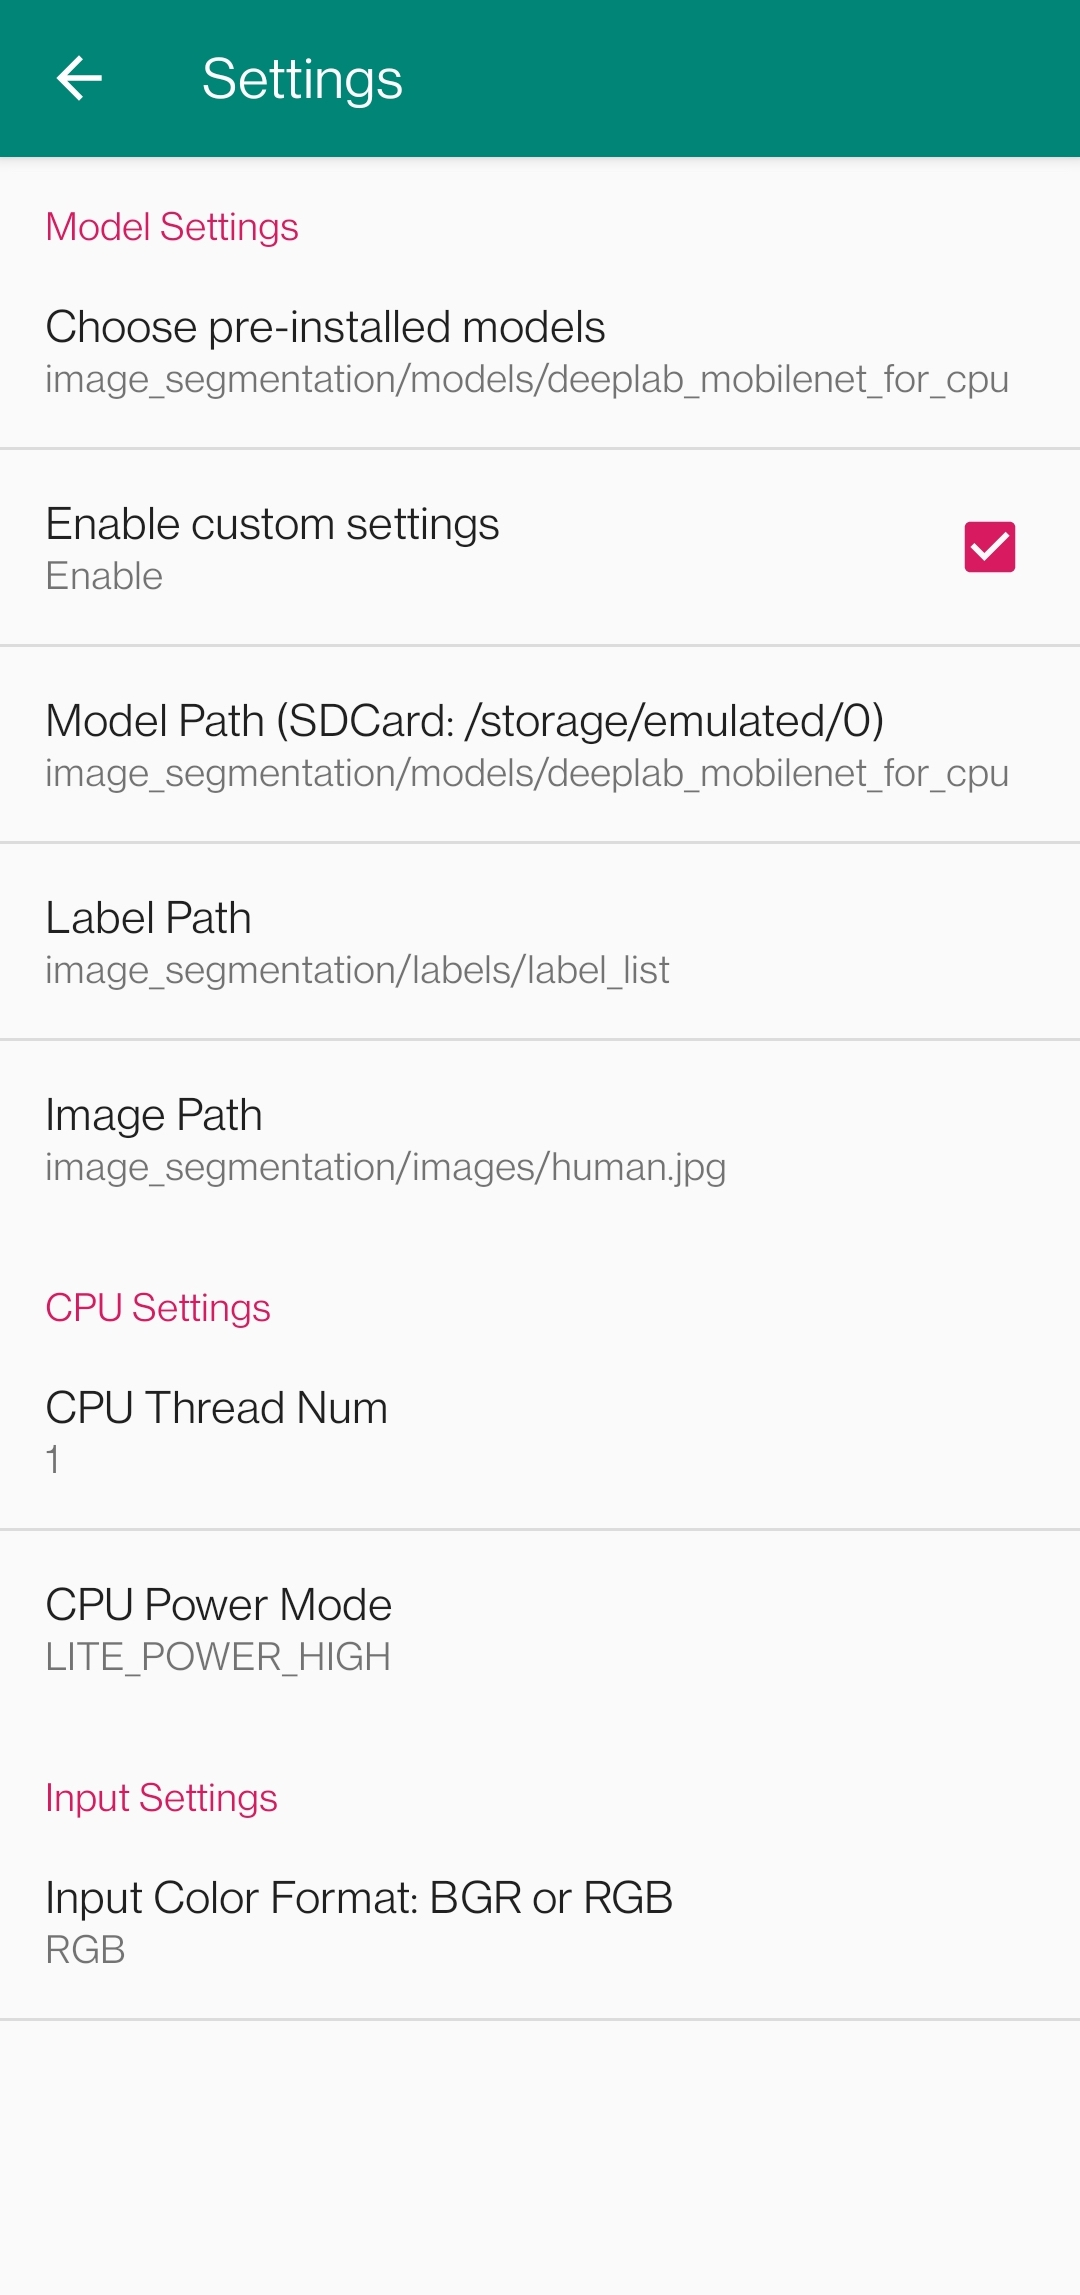
\includegraphics[width=1\textwidth]{figures/settings.jpg}
        \caption{The Whole Settings Page}\label{settings}
    \end{subfigure}
    \begin{subfigure}[t]{0.4\linewidth}
        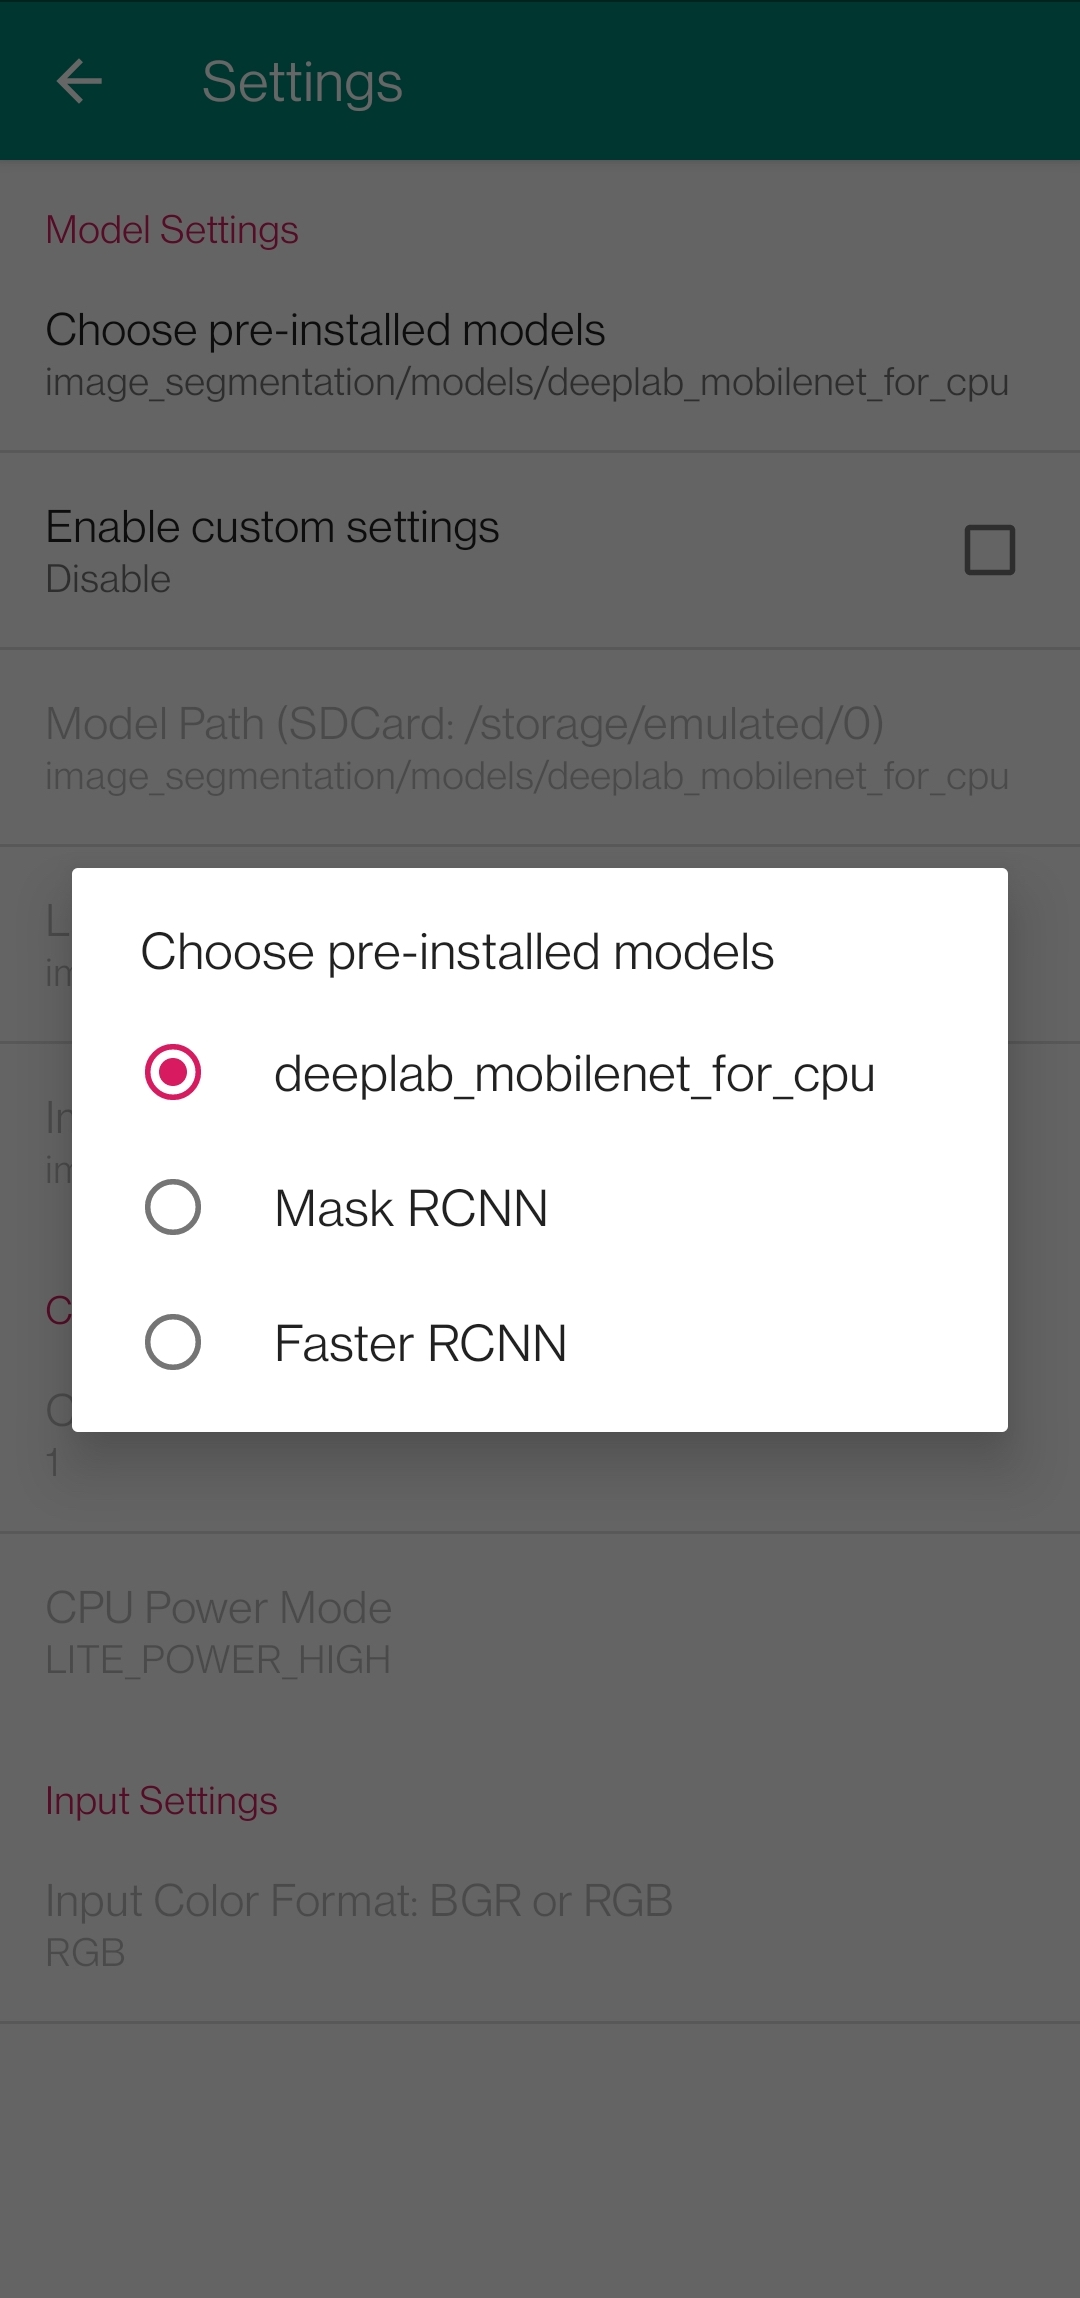
\includegraphics[width=1\textwidth]{figures/type.jpg}
        \caption{Selection Setting about Pre-installed Models}\label{type}
    \end{subfigure}
    \caption{Settings Pages}\label{result1}
\end{figure}


\begin{figure}[htbp]
    \centering
    \begin{subfigure}[t]{0.3\linewidth}
        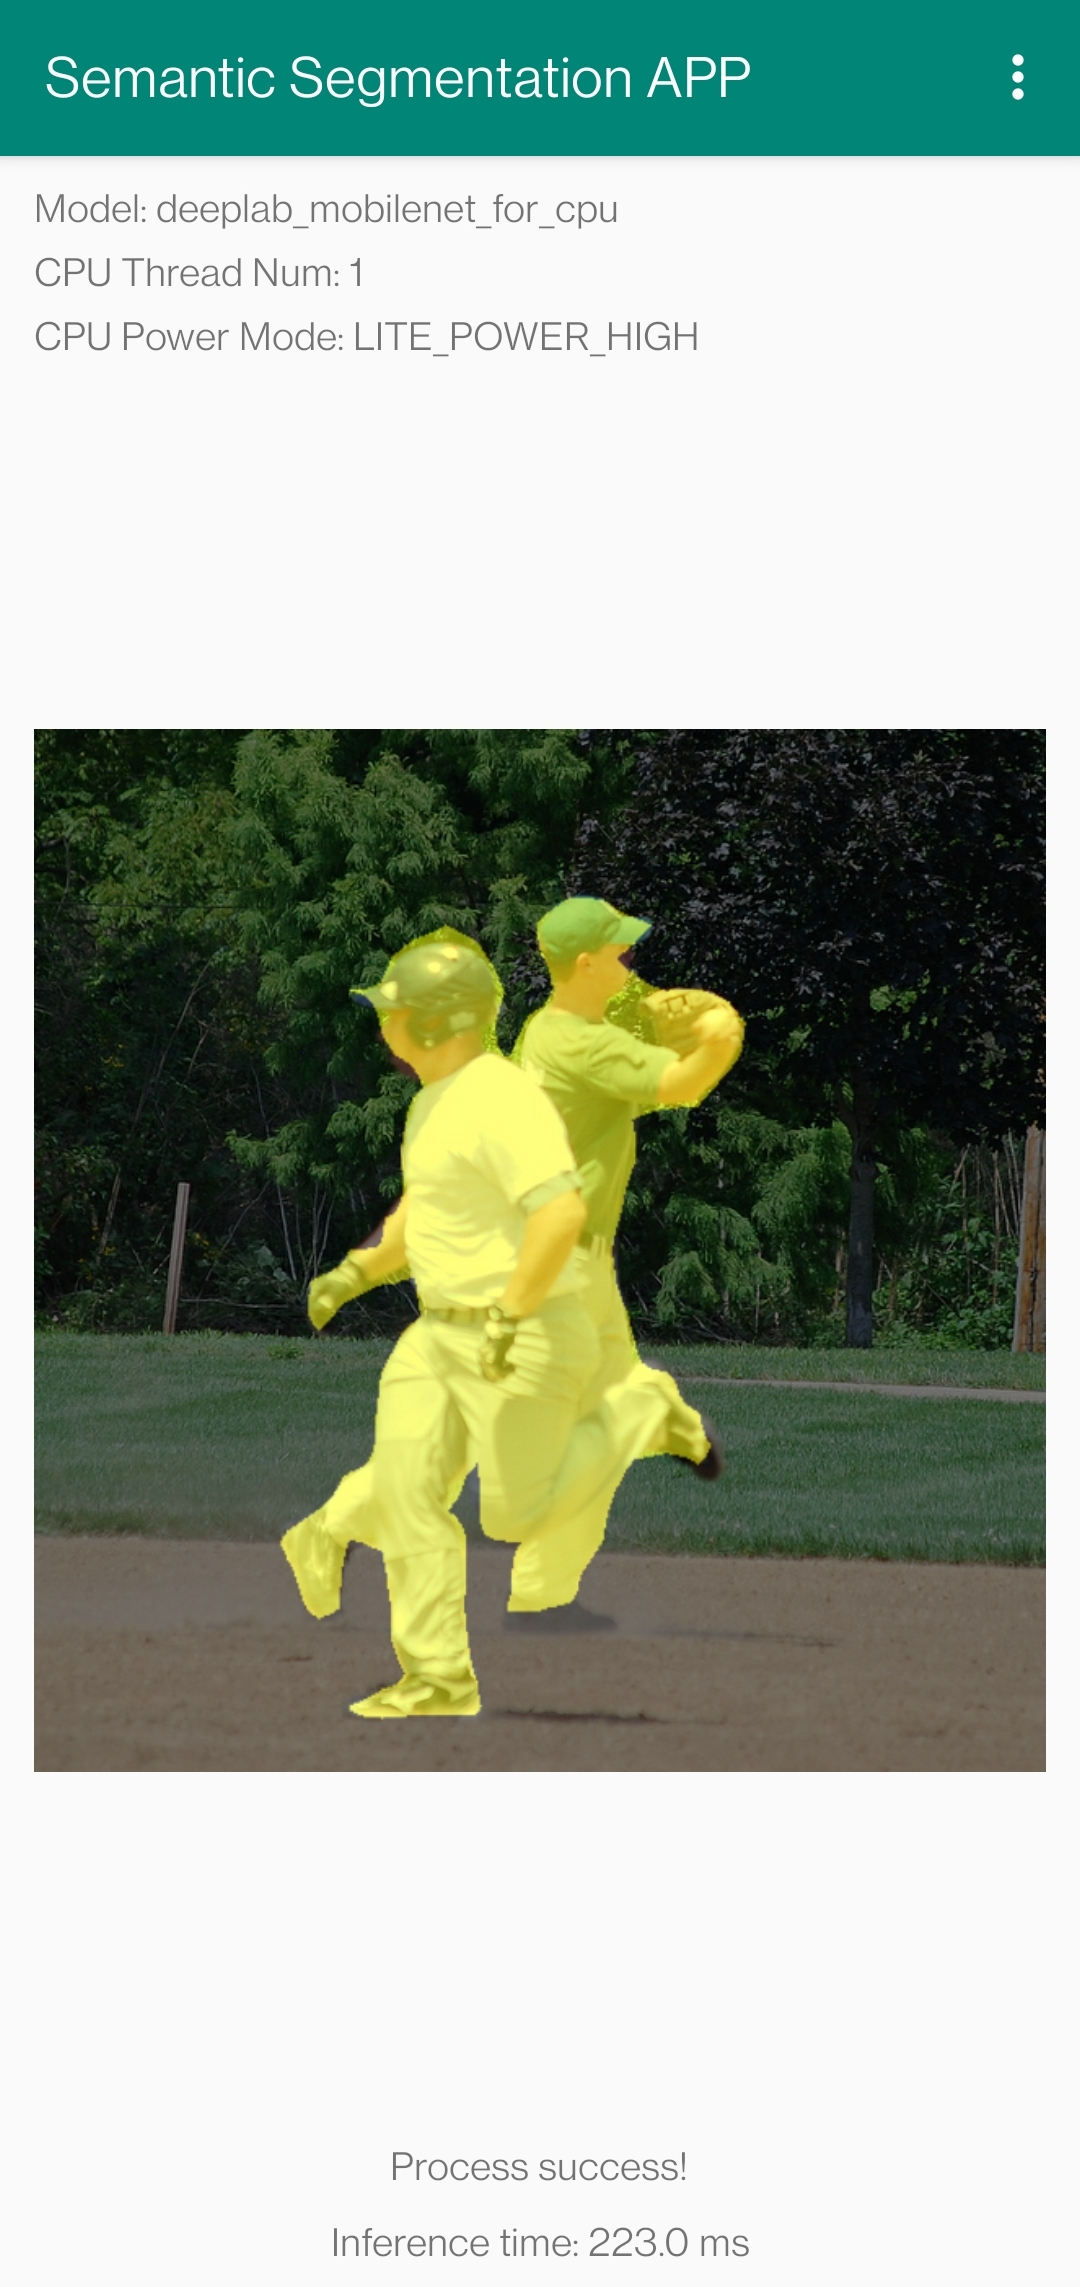
\includegraphics[width=1\textwidth]{figures/paddleresult.jpg}
        \caption{待改}\label{resultpaddle}
    \end{subfigure}
    \begin{subfigure}[t]{0.3\linewidth}
        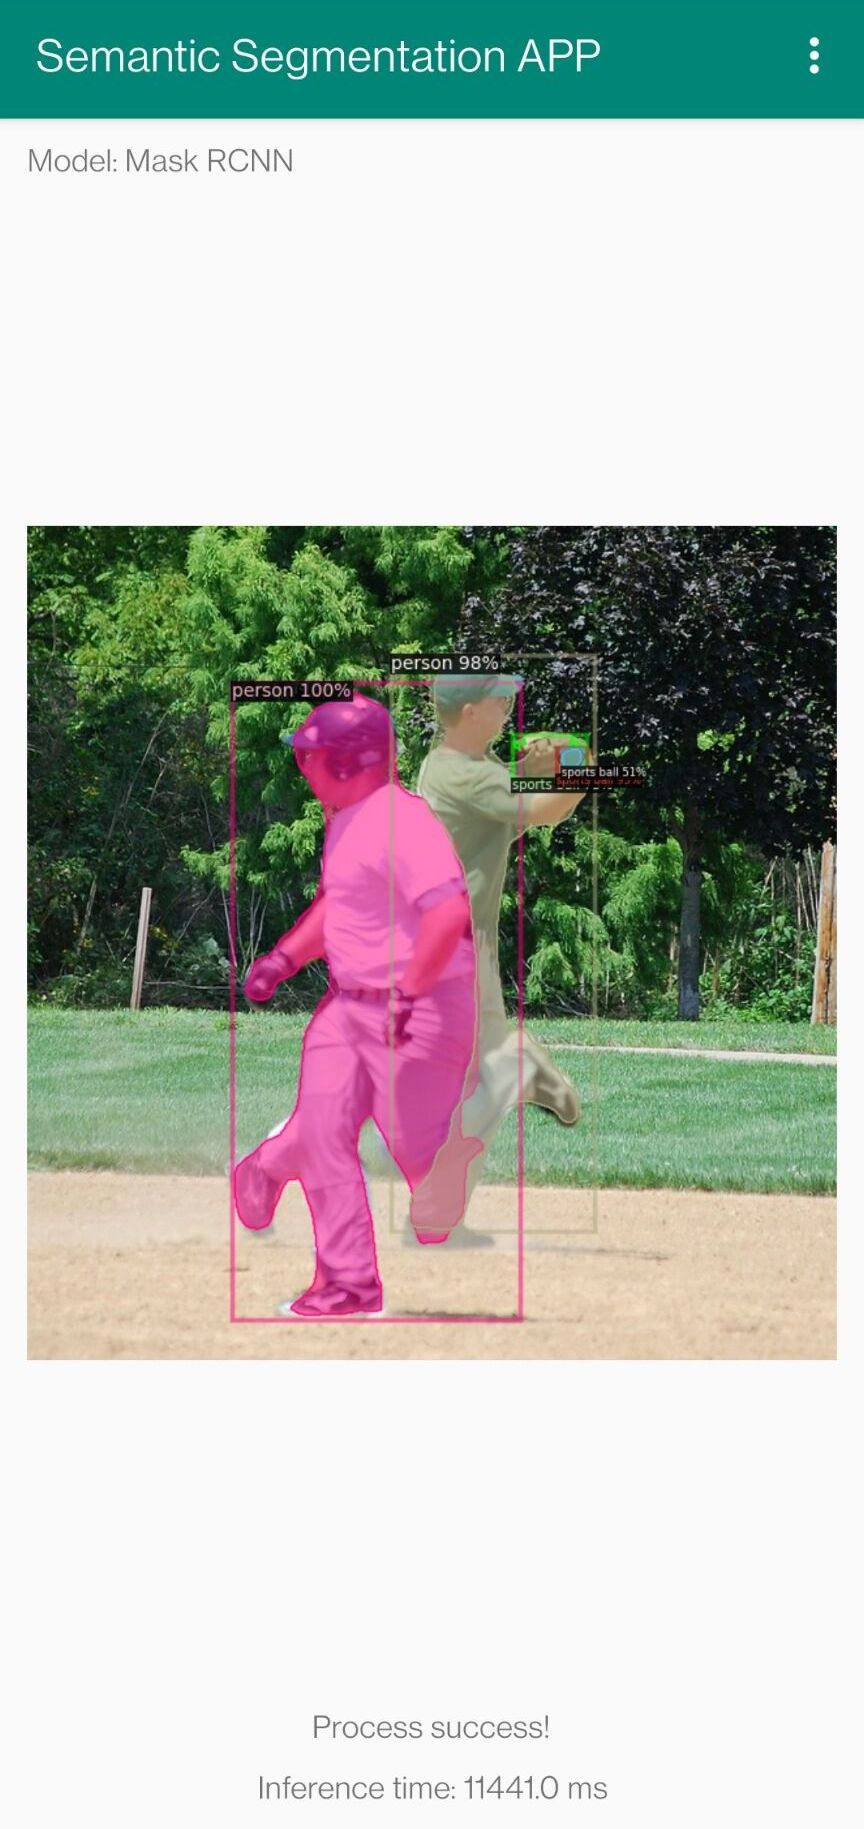
\includegraphics[width=1\textwidth]{figures/maskresult.jpg}
        \caption{待改
        }\label{resultmaskrcnn}
    \end{subfigure}
    \begin{subfigure}[t]{0.3\linewidth}
        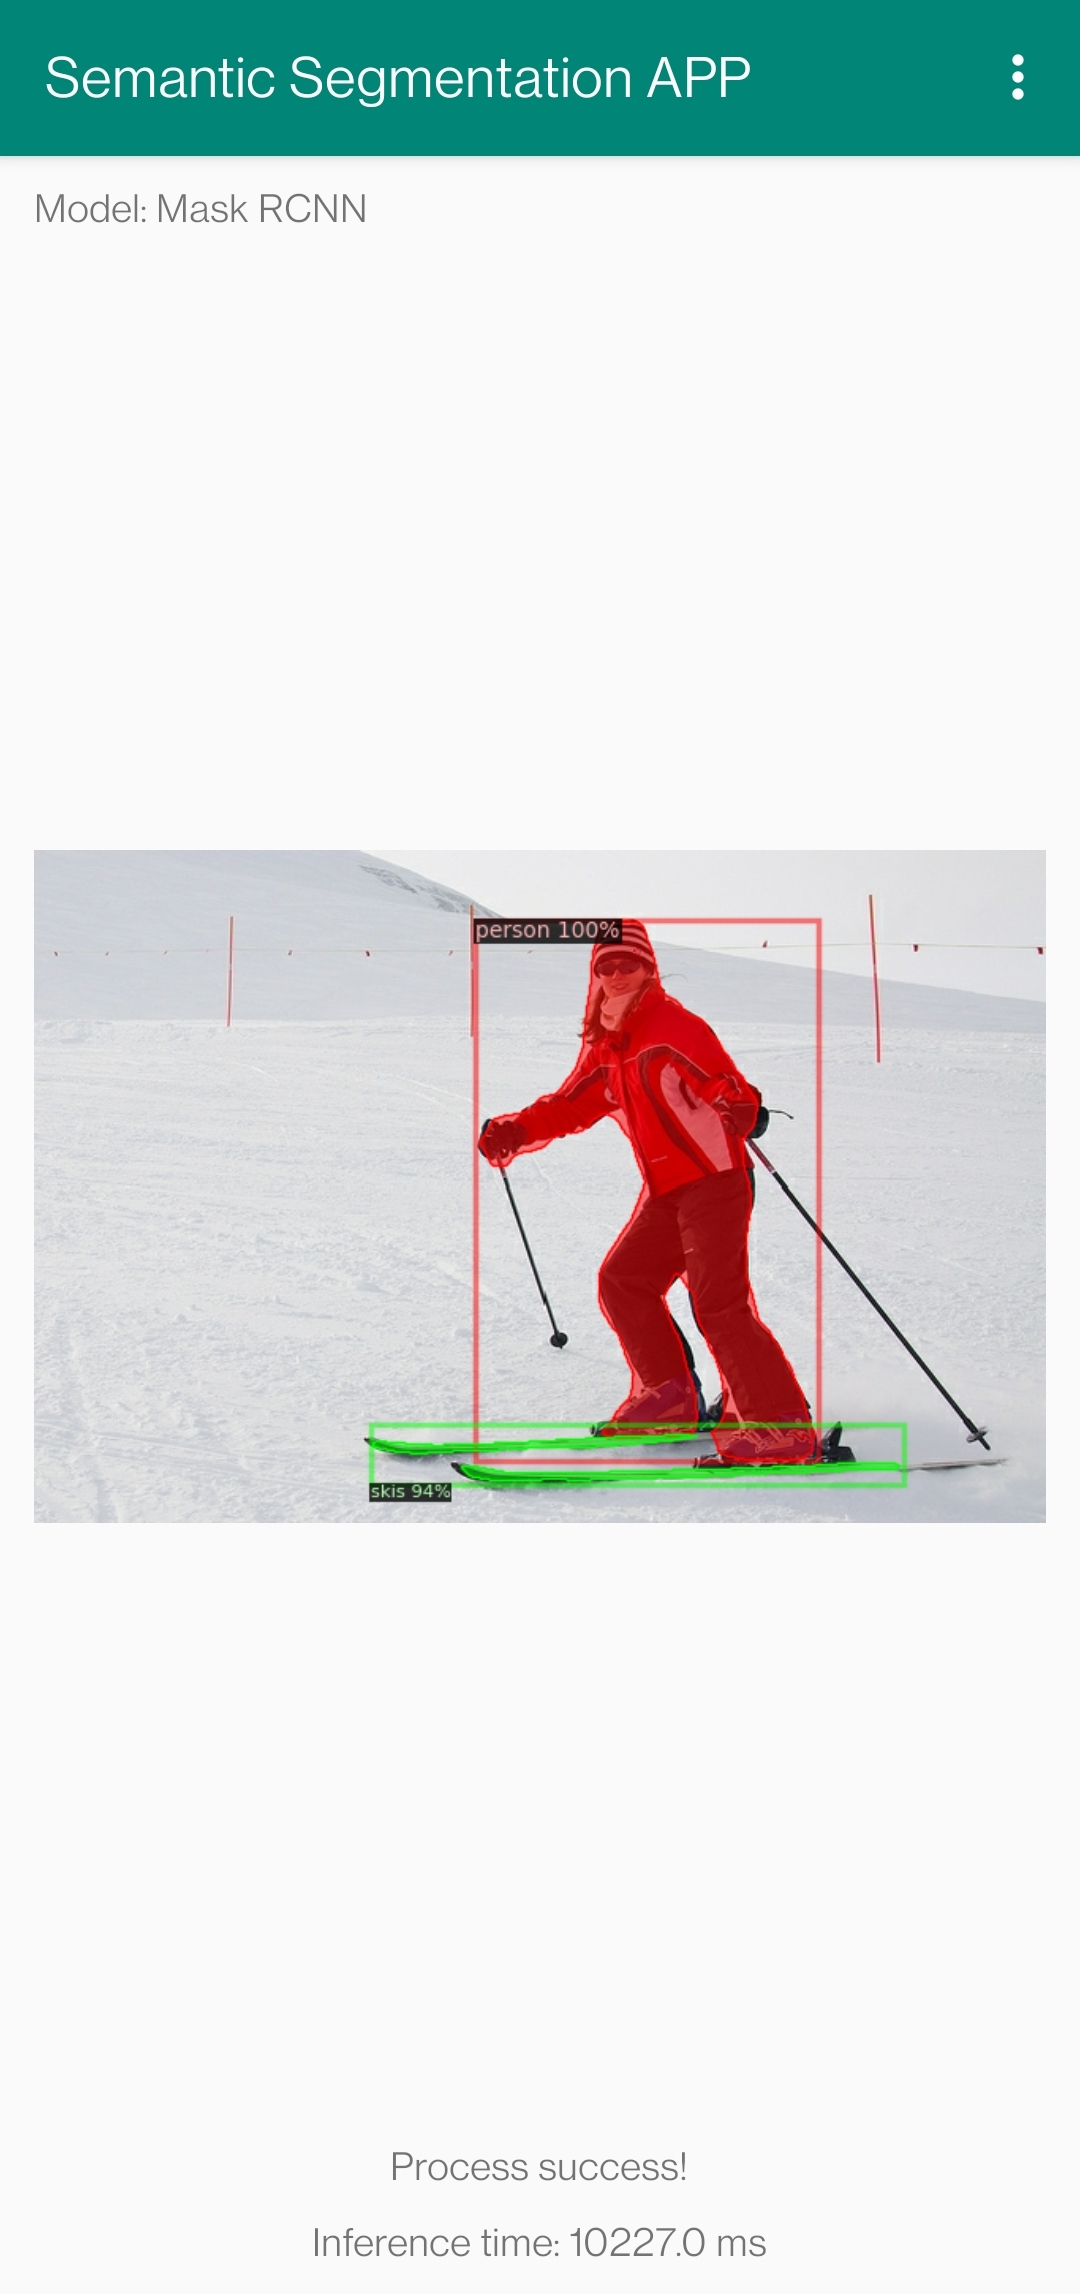
\includegraphics[width=1\textwidth]{figures/ski.jpg}
        \caption{待改}\label{resultskimaskrcnn}
    \end{subfigure}
    \caption{待改}\label{result2}
\end{figure}

%该部分选取了APP的设置页面和分割结果予以展示。设置页面提供了对于模型的选项,用户可以在设置页面里选择模型的路径,图像的路径和通道顺序等等。对于结果来说,可以看到对于物体及其边界的识别的效果较好,而对于实力分割中同类的存在重叠物体的边界识别还存在问题。但是对于单独物体的识别和分割的效果较好,达到了预期。

This part selects the settings page of the APP and the segmentation results to display. The settings page provides options for the model, the user can choose the path of the model, the path of the image and the channel order, etc. on the settings page. For the results, it can be seen that the recognition of objects and their boundaries is better, but there are still problems in the recognition of the boundaries of overlapping objects of the same kind in strength segmentation. However, the effect of recognition and segmentation of individual objects is better, which has reached the expectation.

%其中可以看到在使用非预移植模型时,处理所需的时间较长。其中对于尺寸较大的图片,80%左右的时间用于数据传输,10%左右的时间用于加载模型,10%左右的时间用于分割。对于尺寸较小的图像也仅有50%的时间是真正用于模型的运行。模型运行的效率约为$2s/Obj$

It can be seen that the processing time is longer when using the non-preported model. Among them, for large-sized images, about 80\% of the time is used for data transmission, about 10\% of the time is used to load the model, and about 10\% of the time is used for segmentation. For smaller images, only 50\% of the time is used for running the model. The model runs with an efficiency of about $2s/Obj$.

%总的来说,本论文在Faster R-CNN和Mask R-CNN和FaPN模型的训练结果上取得了不逊于原论文的结果,并部署在了服务器端。在与移动端模型相比较时,在模型加载速度和效率上略逊于移动端模型,但在分割效果,特别是对于小物体和物体边缘的分割上取得了显著优势。

In general, this paper achieves comparable results to the original paper on the training results of Faster R-CNN, Mask R-CNN, and FaPN models, which are deployed on the server-side. When compared with the mobile-end model, the model loading speed and efficiency are slightly inferior to the mobile-end model, but it has achieved significant advantages in segmentation effect, especially for the segmentation of small objects and object edges.

\subsection{Environment}

\begin{itemize}
    \item \textbf{Model training environment: }
    
    1 Intel(R) Xeon(R) Gold 6226 CPU @ 2.70GHz

    2 NVIDIA GeForce RTX 2080Ti graphics cards

    Torch version: 1.7.1+cu101

    Python 3.6.9
    \item \textbf{Model running environment: }

    待改为Jetson Nano

    1 Intel(R) Xeon(R) Platinum 8255C CPU @ 2.50GHz

    No GPU

    Torch version: 1.8.0+cpu

    Python 3.8.10

    \item \textbf{Other Tools Used: }
    
    \href{https://github.com/HarisIqbal88/PlotNeuralNet}{PlotNeuralNet} \cite{plotNeuralNet}

    \href{https://github.com/facebookresearch/detectron2}{detectron2} \cite{wu2019detectron2}


\end{itemize}


\clearpage
% !Mode:: "TeX:UTF-8"
% !TEX program  = xelatex
\section{Conclusion and Future Work}
%In this paper, we illustrated the construction of our trajectory dataset from raw GPS data. Then we proposed the concept of trajectory-based road correlation and built a trajec- tory next-hop model to learn road embeddings and calculate road correlation matrix. Based on that, we gave the theory of refined adjacency matrix and integrated it into SOTA traf- fic prediction models to improve their performance. Extensive experiment results proved the effectiveness and robustness of our models. Following, a case study demonstrated the rationality of the road correlation.
%However, the road correlation matrix C is still a static representation of the road net- work graph. To strengthen its temporality, we are planning to extend our current work to study time-varying road correlations by splitting C into 24 hours and build a time-dynamic traffic prediction model.


%本文主要成果是复现了FaPN一文的实验结果并在COCO 2017和TT100K数据集上取得了分割结果。可以得出结论,FaPN中的FSM和FAM模块可以提升对于小物体和物体边界的预测性能,具有在原有模型基础上进一步提升效果的功能。本文将其实用化,包装为Android APP,将前后端进行解耦,实现了模型的通用化和模块化,提高了模型的实用性。

The main result of this paper is to reproduce the experimental results of the FaPN paper and obtain segmentation results on the COCO 2017 and TT100K datasets. It can be concluded that the FSM and FAM modules in FaPN can improve the prediction performance of small objects and object boundaries, with the function of further improving the effect based on the original model. This article puts it into practical use, packages it as an Android APP, decouples the front and back ends, realizes the generalization and modularization of the model, and improves the practicality of the model.

%其中对于服务器端模型的训练结果,在相同训练参数和环境的情况下达到了原模型FaPN的参考值,其相对于FPN网络有0.3\%到1.2\%不等的提升,特别是证明了在对于模型边界和小物体的预测上的提升。说明了选择模块和对齐模块的有效性。对于APP的最终结果,其应用了预训练的Mask RCNN和 Faster RCNN模型和移动端Paddle Lite模型,并在物体分割的问题上取得了较好的结果,在排除网络传输和模型加载的时间后,移动端Paddle Lite模型对于单张图片的分割结果平均在200ms,但因为其所调用的是移动端的AI推理引擎,限于计算力,分割结果与部署在服务端的模型仍存在差距。服务端的模型的平均分割时间在2s/Obj,但分割结果相对于移动端模型更精确,能识别的物体类型也更加丰富。

The training results of the server-side model have reached the reference value of the original model FaPN under the same training parameters and environment. Compared with the FPN network, it has an improvement ranging from 0.3\% to 1.2\%. Improved prediction of model boundaries and small objects. Illustrates the effectiveness of feature selection modules and feature alignment modules. For the final result of the APP, it applied the pre-trained Mask RCNN and Faster RCNN models and the mobile Paddle Lite model and achieved good results in the problem of object segmentation. After excluding the time of network transmission and model loading, The average segmentation result of the mobile Paddle Lite model for a single image is $200ms$, but because it calls the AI inference engine on the mobile side and is limited in computing power, there is still a gap between the segmentation results and the model deployed on the server-side. The average segmentation time of the server-side model is $2s/Obj$, but the segmentation results are more accurate than the mobile-side model, and the types of objects that can be recognized are also more abundant.

%但本文还存在诸多问题,比如模型可供选择的选项较少,训练的迭代次数较少导致无法完全复现原文的结果。由于服务器带宽问题,单张图像处理所需要的时间较长,并且无法实现实时分割的功能。APP的功能较为单一而且界面美观性较差等等。

However, there are many problems in this article, such that the model has fewer options to choose from, and the number of iterations of training is small, resulting in the inability to fully reproduce the results of the original text. Due to server bandwidth issues, single image processing takes a long time and the function of real-time segmentation is not possible. The function of the APP is relatively single, the interface is poorly aesthetically pleasing.\clearpage

\Reference
  \printbibliography[heading=none]\clearpage
% \附录
%   % !Mode:: "TeX:UTF-8"
% !TEX program  = xelatex
\section*{数据获取函数}\label{A:data}
\Python{utils.py}{code/examples/utils.py}
\clearpage
% \Acknowledgments
%   % !Mode:: "TeX:UTF-8"
% !TEX program  = xelatex
Firstly, I would like to give my heartfelt thanks to my parents for decades of nurturing, you built the foundation of all my life.

Sincere gratitude should also go to the EMI group and all the members for the selfless help on academic, especially to Prof. Ran Cheng, Prof. Qi Hao, Dr. Shihua Huang and Dr. Gongjin Lan.

I also have to express my appreciation to all my friends who helped me in my tough time, my old friends, Xuechen, Chenyu, Hao, Xinyue and much more, thanks for the company. Also to all the members of CUI Lab, Haotian Gao, Yuchen Wang, Yusong Cui and Zheng Dong. My friends Yutao Pan, Zijian Chen, Weicheng Wu, Yitong Zheng who have accompanied me for four years and anyone who have ever helped me.


% My little princess wolf, special thanks for you. Wish you and other four girls stay positive and be happy for good. 


\end{document}
